% ======================================================================
% GiTrip Final Report
% Author: Tatsunori Ono
% Degree/Year: 3rd Year Computer Science
% Supervisor: Professor Mike Joy
% Academic Year: 2025/26
%
% Based on the University of Warwick CS Report Template
% Original template by Chris Quinn 28/06/2020
% ======================================================================

\documentclass[pdftex,11pt,a4paper,oneside]{report}

% -- Original Warwick template packages -----------------------------------
\usepackage{amsmath}
\numberwithin{equation}{chapter}
\usepackage{algorithm}
\usepackage{algpseudocode}
\usepackage{listings}
\lstset{
  basicstyle=\ttfamily\small,
  keywordstyle=\bfseries,
  commentstyle=\itshape\color{gray},
  numbers=left,
  numberstyle=\tiny\color{gray},
  numbersep=6pt,
  frame=single,
  breaklines=true,
  xleftmargin=1.5em,
  framexleftmargin=1.5em,
}
\usepackage{fancyhdr}
\usepackage{graphicx}
\usepackage{setspace}                 % Spacing (used on front page for crest)
\usepackage[]{fncychap}     % Warwick-style chapter headings
\usepackage[hyphens]{url}
\usepackage{xcolor}
\usepackage{tabularx}
\usepackage{appendix}
\usepackage{cite}                     % IEEE citation grouping [1]-[3]

% -- TikZ for UML class diagram -------------------------------------------
\usepackage{tikz}
\usetikzlibrary{positioning, arrows.meta, calc, fit, shapes.geometric}

% -- Additional packages for GiTrip content -------------------------------
\usepackage[a4paper,margin=2.5cm]{geometry}
\usepackage{microtype}
\usepackage{lmodern}
\usepackage{float}
\usepackage{caption}
\usepackage{subcaption}
\usepackage{booktabs}
\usepackage{longtable}
\usepackage{array}
\usepackage{multirow}
\usepackage{pdfpages}

% Keep hyperref last
\usepackage[hidelinks]{hyperref}

% -- Paragraph formatting -------------------------------------------------
\setstretch{1.15}
\setlength{\parskip}{0.35em}
\setlength{\parindent}{0pt}

% -- Warwick-style header/footer (from original template) -----------------
\fancyhf{}
\pagestyle{fancy}
\renewcommand{\headrulewidth}{0.2pt}
\fancyhead[L]{\leftmark}
\fancyhead[R]{CS310 Computer Science Project}
\lfoot{\centering \thepage}

%%%%%%%%%%%%%%%%%%%%%%%%%% DOCUMENT STARTS %%%%%%%%%%%%%%%%%%%%%%%%%%%%%

\begin{document}

% Front Matter (excluded from word count)
% !TEX root = ../Report.tex

\thispagestyle{empty}

\begin{spacing}{2}
    \begin{center}
        
\includegraphics[scale=0.45]{Preamble/WarwickCrest.pdf}
        % Two options: WarwickCrest.pdf (colour) or WarwickAlt.pdf (B&W)
    \end{center}
    \vspace{5mm}
    \begin{center}
        \textbf{\begin{LARGE}
        GiTrip \\ $\sim$\textit{Git} for Collaborative Trip Planning$\sim$
        \end{LARGE}}
        \vspace{5mm}
    \end{center}
    \begin{center}
        {\large CS310 Computer Science Project}\\
        \vspace{20mm}
    \end{center}
    \begin{center}
        \textbf{\large Tatsunori Ono}
        \vspace{20mm}
    \end{center}
    \begin{center}
        {\large Supervisor: Professor Mike Joy}\\
        {\large Second Assessor: Professor Charilaos Efthymiou}\\
        \vspace{5mm}
        \textbf{\large Department of Computer Science}\\
        {\large University of Warwick}\\
        {\large Academic Year 2025/26\\}
    \end{center}
\end{spacing}

\pagenumbering{roman}

% !TEX root = ../Report.tex
\chapter*{Abstract}
\addcontentsline{toc}{chapter}{Abstract}

Trip planning becomes significantly more complex when multiple people collaborate,
because itineraries evolve through parallel edits, last-minute changes, and
disagreements about priorities. Existing tools typically optimise a single
itinerary (e.g., mapping and routing applications) or support generic
collaboration (e.g., shared documents), but they do not provide robust
change-management semantics tailored to itineraries. This project presents
\textit{GiTrip}, a server-rendered web application that applies Git-style
version control concepts to trip planning: a trip is modelled as a repository,
alternative itineraries are branches, each saved version is a commit containing
a complete snapshot, and divergent branches can be merged using a three-way
merge with an explicit conflict-resolution user interface.

GiTrip integrates routing, scheduling constraints, and usability-focused
interaction. An automatic scheduler produces feasible multi-day itineraries
based on user inputs such as active hours, stay durations, ordering constraints,
desired time windows, public transit selection, and opening hours. Users can
then refine plans using two interactive surfaces: a timeline editor for
adjusting arrival/departure times and a map editor for repositioning locations.
To address the usability barrier of Git concepts for non-technical users, GiTrip
includes an ``Easy mode'' that hides advanced controls while preserving version
safety.

The completed system was evaluated through an in-person Evaluation Day
demonstration and user acceptance testing. Objective task results show high
completion rates for auto-scheduling feasibility and merge conflict resolution,
with qualitative feedback highlighting the novelty and usefulness of
version-controlled planning. The report details the requirements, system design,
implementation, testing strategy, and evaluation outcomes, and concludes with
limitations and future work (including optional machine learning extensions
beyond the original project scope).

\vspace{0.6em}
\textbf{Keywords:} trip planning; version control; branching and merging;
scheduling constraints; routing; usability; progressive web app; conflict
resolution

% !TEX root = ../Report.tex
\chapter*{Acknowledgements}
\addcontentsline{toc}{chapter}{Acknowledgements}

I would like to thank my supervisor, Professor Mike Joy, for his consistent
guidance throughout the entire project, constructive feedback from the initial
planning and the Project Specification through to the Progress Report and Final
Report, and regular supervision meetings that kept the project on track. I also thank my second assessor,
Dr Charilaos Efthymiou, for his feedback on the Progress Report which helped
refine the evaluation approach and the presentation of technical material. I
thank Dr Greg Watson for organising the CS310 module, delivering the supporting
lectures, and coordinating Evaluation Day logistics. I thank all participants
who completed the preliminary survey and those who attended (or responded
remotely to) the Evaluation Day survey and user acceptance tests; their time and
feedback directly improved the usability and robustness of GiTrip. I am
grateful to my friends, family, and partner for their ongoing support and
motivation throughout the project. Finally, I am deeply grateful
to my late father, who encouraged me to pursue my studies at the University of
Warwick.
% !TEX root = ../Report.tex
\chapter*{Abbreviations}
\addcontentsline{toc}{chapter}{Abbreviations}

\begin{longtable}{@{}p{0.20\linewidth}p{0.75\linewidth}@{}}
\toprule
\textbf{Term} & \textbf{Meaning} \\
\midrule
API   & Application Programming Interface \\
CRDT  & Conflict-free Replicated Data Type \\
CSP   & Content Security Policy \\
DAG   & Directed Acyclic Graph \\
DP    & Dynamic Programming \\
EJS   & Embedded JavaScript Templates \\
GDPR  & General Data Protection Regulation \\
HTTP  & Hypertext Transfer Protocol \\
iCal / ICS & iCalendar format / calendar file \\
JSON  & JavaScript Object Notation \\
LCA   & Lowest Common Ancestor (in a commit graph) \\
LLM   & Large Language Model \\
NN    & Nearest Neighbour (heuristic) \\
ORS   & OpenRouteService \\
PWA   & Progressive Web App \\
SQL   & Structured Query Language \\
SUS   & System Usability Scale \\
TAM   & Technology Acceptance Model \\
TSP   & Travelling Salesman Problem \\
UI/UX & User Interface / User Experience \\
WCAG  & Web Content Accessibility Guidelines \\
\bottomrule
\end{longtable}

% !TEX root = ../Report.tex
\tableofcontents
\listoffigures
\listoftables

% !TEX root = ../Report.tex
% Lists are included in Contents.tex for this report.
% This file is retained for template compatibility.

% !TEX root = ../Report.tex
\clearpage
\pagenumbering{arabic}


% Main Body
% !TEX root = ../Report.tex
% ======================================================================
\chapter{Introduction}
\label{ch:intro}
% ======================================================================

This report presents the design, implementation, testing, and evaluation of GiTrip, a web application for collaborative trip planning via Git~\cite{ref_git}-style version control system (VCS) combined with constraints-aware auto-scheduler.

\section{Problem Context and Motivation}
Trip planning is time-consuming because a feasible schedule must satisfy
multiple constraints simultaneously, including travel time between destinations,
opening hours, stay durations, and daily activity limits. The process becomes
more complex for group trips, where participants propose alternative routes and
schedules, with edits often distributed across chat messages, screenshots, and
shared documents. This fragmented approach increases the
likelihood of duplicated work, accidental overwrites, and loss of rationale for
changes.

While existing route planners can optimise a single itinerary and generic collaboration tools can support shared documents, optimising the entire trip schedule and supporting change management in group trip planning remain insufficient.

To validate the practical relevance of this problem, a preliminary survey was
conducted with 30 participants (full questionnaire and results in Appendix~\ref{appx:prelim_survey}).
Key findings support three observations:
\begin{enumerate}
  \item \textbf{Planning is widely effortful:} 60\% (18/30) reported trip
        planning as \textit{often} or \textit{always} stressful/time-consuming; 93\% (28/30) as
        \textit{at least sometimes} stressful.
  \item \textbf{Fragmented tool usage is common:} 83\% (25/30) use Google
        Maps~\cite{ref_google_maps} for planning; 47\% (14/30) use Google Docs~\cite{ref_google_docs}/Microsoft Word~\cite{ref_ms_word}
        (multi-select). Current practice fragments planning across maps and
        general-purpose documents.
  \item \textbf{Demand for an integrated solution:} 90\% (27/30) responded
        \textit{very likely} or \textit{somewhat likely} to use GiTrip.
\end{enumerate}
These findings, initially presented in the Progress Report, motivated the
background research and competitor analysis in
Chapter~\ref{ch:background}.

\section{Project Overview}
GiTrip applies Git-style VCS semantics to trip planning. A trip is represented as a repository containing the users’ commits (changes made to the trip). Users can branch (make alternative routes) and merge branches via structured conflict resolution to make the final trip plan. This version-controlled plan is integrated with an automatic scheduler that produces a non-overlapping itinerary while respecting constraints such as active hours, per-stop stay duration, user preferences, and opening hours.

The key design goal is usability for non-experts. Git concepts are surfaced through a clear web interface (buttons for branching/merging, workflow graph, conflict resolver screens). Trip plans are visualised using an interactive timeline (editable by dragging) and a map view showing ordered stops and route geometries. The ``Git mode'' toggle, when turned off, hides Git-specific vocabulary for non-technical users. The feature-ranking results (Q5) of the survey reinforce this requirement: concrete itinerary features such as timeline/map visualisation, travel-time estimation, and automatic optimisation are perceived as most helpful, while Git-style trip repository concepts are less directly valued by some respondents (Appendix~\ref{app:agg-res}). Therefore, Git-style semantics should be implemented to enable VCS, but presented through an approachable interface that does not assume prior Git knowledge.

\section{Objectives and Significance}

The objectives, categorised by MoSCoW (Must/Should/Could/Won't) prioritisation, were initially formalised in the Project Specification. Must-have objectives include covering repository history,
an optimised automatic scheduler, routing integration, interactive
visualisation, and merging with conflict resolution. The full requirements and
their rationale are detailed in Chapter~\ref{ch:requirements}.

GiTrip is a suitably challenging 3rd-year Computer Science project because it combines: (i) VCS semantics over structured data, (ii) constraint-aware scheduling with external routing services, and (iii) interactive visualisation with editable timelines and maps. The project makes a novel contribution by applying VCS semantics to collaborative trip planning, addressing a documented gap in existing tools that are further discussed in Chapter~\ref{ch:background}. This is also significant because the combination of constraint-aware scheduling with structured change management has potential applications beyond tourism when generalised, including project planning and resource allocation scenarios.
% !TEX root = ../Report.tex
% ======================================================================
\chapter{Background and Related Work}
% ======================================================================

This chapter positions GiTrip within existing trip-planning and collaboration
tooling, and introduces foundational techniques used in the system: version
control semantics, scheduling heuristics, string matching, accessibility
heuristics, and relevant web standards.

\section{Trip Planning and Routing Tools}
Most users plan trips using mapping and routing tools such as Google Maps and
Apple Maps \cite{ref_google_maps,ref_apple_maps}. These applications provide
high-quality route computation and support multiple transport modes, but their
data model is fundamentally \textit{single-plan centric}. Users can create lists
and saved routes, but they cannot easily branch into alternative itineraries,
compare versions, and merge parallel edits with structured conflict handling.

Public-transport-focused tools such as Citymapper offer strong transit routing
and navigation \cite{ref_citymapper}, but similarly treat the itinerary as an
output rather than a version-controlled artefact. Trip planning products such as
Wanderlog, Furkot, Roadtrippers, and TripIt provide itinerary management
features and collaboration to varying degrees
\cite{ref_wanderlog,ref_furkot,ref_roadtrippers,ref_tripit}, yet they generally
emphasise itinerary presentation and booking integration rather than explicit
version control semantics. Google Travel aggregates trip components and
suggestions but does not provide Git-style change management
\cite{ref_google_travel}.

GiTrip's differentiation is therefore not \textit{better routing} than these
tools; instead, it provides structured change management and alternative
exploration, paired with sufficient routing and scheduling integration to keep
plans feasible.

\section{Generic Collaboration Tools}
When collaboration is required, users commonly use documents and spreadsheets to
manage itineraries: Google Docs/Sheets, Microsoft Word/Excel, and increasingly
general workspaces like Notion
\cite{ref_google_docs,ref_google_sheets,ref_ms_word,ref_ms_excel,ref_notion}.
These platforms have excellent collaboration features but treat an itinerary as
unstructured text or loosely structured tables. As a result, they cannot
automatically recompute travel times after edits, offer interactive map or
timeline visualisation, detect domain-specific conflicts such as overlapping
times, or provide branching semantics for exploring alternatives.

GiTrip's objective is to bring the strengths of version control
(branching/merging/history) into a domain-specific planner where plans are
first-class structured data.

\section{Version Control Concepts and Applicability}
Git is the dominant distributed version control system in software development
\cite{ref_git}. Its key semantics include commits (immutable versions), branches
(named pointers to commits), and merges (reconciling divergent commit histories).
Git's internal model stores snapshots rather than deltas: each commit represents
a complete view of the repository state \cite{ref_progit_snapshots}. This is
particularly relevant for GiTrip because a trip plan can be represented naturally
as a JSON document. Snapshot storage enables instant branch switching (render the
head snapshot), version restoring (create a new commit from an older snapshot),
and three-way merges (compare a base snapshot against two branch snapshots).

However, applying Git semantics to structured itinerary data introduces
challenges: traditional line-based diff/merge strategies (e.g., \texttt{diff3})
are designed for text and can produce poor results for structured JSON. The
fundamental three-way merge idea remains useful: derive changes in two branches
relative to a common ancestor and combine them, surfacing conflicts when both
sides change the same part incompatibly. Formal work on \texttt{diff3} analyses
its behaviour as a widely used three-way merge algorithm \cite{ref_diff3_paper}.

GiTrip therefore adapts the three-way merge concept to structured itinerary
objects rather than line-based text.

\section{Scheduling and Route Optimisation}
A key sub-problem in trip planning is ordering stops efficiently. This relates to
the Travelling Salesman Problem (TSP), which is computationally hard in general
and commonly addressed with heuristics
\cite{ref_tsp_study,ref_tsp_local_search}. GiTrip uses heuristics that provide
good-enough results for interactive planning rather than exact optimal solutions,
which aligns with practical timetabling and scheduling approaches discussed in
the automated timetabling literature \cite{ref_patat}.

For example, the Nearest Neighbour (NN) heuristic greedily selects the closest
next stop and is a common baseline; it is known to be simple and fast while not
always optimal \cite{ref_nn_tsp}. GiTrip also includes an educational algorithm
visualisation that demonstrates NN, NN + 2-opt improvement
\cite{ref_nn_2opt_hybrid}, and Held-Karp
dynamic programming for small instances, helping explain why the production
scheduler uses heuristics.

\section{Approximate String Matching for Place Search}
Place search relies on external geocoding and search services (e.g., Nominatim).
Returned results can be noisy or differently formatted across user inputs. GiTrip
improves usability by re-ranking candidates using approximate string matching,
normalising input strings and applying edit distance techniques
\cite{ref_navaro_string_matching}. This improves the ``easy add'' flow where
users paste free-form place names and expect robust matching.

\section{Structured Data Merge and JSON Patch Formats}
JSON-based systems frequently represent updates using patch formats. RFC 7396
(JSON Merge Patch) defines a merge-based approach for describing modifications
to JSON objects \cite{ref_rfc7396}. However, general-purpose patch formats do
not provide domain-specific semantics for itineraries: for example, they do not
encode constraints such as time overlaps or opening-hours validity. GiTrip
therefore uses a domain-aware merge strategy:
\begin{itemize}
  \item file-like maps (\texttt{snapshot.files}) are merged per-key using deep
        equality,
  \item trip plans (\texttt{snapshot.plan}) are merged per-day and per-stop with
        explicit conflict detection for semantic fields.
\end{itemize}

\section{Usability and Accessibility Frameworks}
GiTrip must balance power-user semantics (branches, merges) with novice
usability. Nielsen's usability engineering framework provides well-established
heuristics for evaluating interfaces and diagnosing common usability problems
\cite{ref_nielsen}. Nielsen's heuristics were preferred over heavier frameworks
because they are practical for small teams, support rapid iteration, and directly
map to UI design decisions such as visibility of system state, consistency, error
prevention, and recognition over recall.

Accessibility was guided by WCAG 2.2 principles \cite{ref_wcag22}, particularly
around keyboard navigation, contrast, and clear labelling. GiTrip's use of
interactive map and timeline components introduces accessibility challenges; this
report therefore discusses mitigations and remaining limitations.

For evaluation, GiTrip used a survey instrument that included the System
Usability Scale (SUS) and Likert-style questions aligned with constructs from the
Technology Acceptance Model (TAM), notably perceived usefulness and perceived
ease of use \cite{ref_tam_davis}. TAM was not used as a strict statistical model
due to limited sample size, but its constructs informed question design and
interpretation.

\section{Summary: Gap in Existing Approaches}
In summary, existing trip planning tools provide routing and itinerary management
but lack robust version control semantics. Existing collaboration tools provide
sharing but lack domain structure. Version control systems provide branching and
merging but do not operate on itinerary semantics. GiTrip's novelty is that it
combines these approaches into a coherent system: a version-controlled,
constraint-aware, user-editable itinerary planner.

% !TEX root = ../Report.tex
% ======================================================================
\chapter{Requirements and Project Specification}
\label{ch:requirements}
% ======================================================================

This chapter describes the requirements that guided GiTrip's development, how
they were derived, and how they map to success criteria and evaluation. It also
documents scope boundaries, including the explicit decision to exclude Artificial Intelligence (AI)-powered
itinerary generation from the Minimum Viable Product (MVP).

\section{Requirements Elicitation}
Requirements were formed using two complementary inputs:
\begin{itemize}
  \item \textbf{Background research} (from Chapter~\ref{ch:background}) into competitor tools (maps, generic collaboration, and trip-planning products) and foundational techniques (version control, scheduling heuristics, etc.).
  \item \textbf{A preliminary survey} (as discussed in Section~\ref{sec:motivation} and Section~\ref{sec:overview}) to understand current trip-planning workflows, perceived pain points, and interest in proposed features.
\end{itemize}

\section{MoSCoW Objectives}
The Project Specification defined MoSCoW objectives. The following is the summary of Must-have (M1--M5) and Should-have (S1--S2) objectives, which formed the MVP definition:

\subsection*{Must-haves (M)}
These five objectives address the core gap identified in Chapter~\ref{ch:background}: no existing tool combines version control, constraint-aware scheduling, visual editing, and structured merging in a single workflow.
\begin{enumerate}[label=\textbf{M\arabic*}]
  \item \textbf{Trip repositories with history:} commits, branches, and snapshot history; visualisation of version history. This directly addresses the lack of change management in existing trip planners (Section~\ref{sec:competitors}).
  \item \textbf{Optimised automatic scheduler:} produce a feasible multi-day plan from places, durations, ordering constraints, desired windows, active hours, breaks, target day ranges, and preferences. The preliminary survey found 60\% of respondents reported planning as often or always stressful, motivating automation of the most tedious step.
  \item \textbf{Routing data integration:} retrieve travel-time data (e.g., OpenRouteService and Google Directions) and feed into scheduling. Without real travel durations, the scheduler cannot produce feasible plans.
  \item \textbf{Interactive visualisation:} timeline and map with editing and committing. The survey's feature ranking (Q5) placed timeline/map visualisation as the most valued capability.
  \item \textbf{Merge and conflicts:} structured merge for plan JSON with a conflict resolver screen. This is the core mechanism that enables collaborative editing without accidental overwrites.
\end{enumerate}

\subsection*{Should-haves (S)}
Should-haves improve the quality of generated plans and the branching workflow but are not essential for a demonstrable MVP:
\begin{enumerate}[label=\textbf{S\arabic*}]
  \item \textbf{Opening-hours validation:} automatic nudge to nearest feasible slot.
  \item \textbf{User preferences:} compact vs.\ sparse scheduling; morning/midday/night focus; recompute travel by mode (driving/walking/cycling/transit).
  \item \textbf{Branch productivity:} create branch from Web UI, compare branches, and fork plan from a public repository.
\end{enumerate}

Several Should-have and Could-have features were also added as direct responses to preliminary survey feedback (Q7 and Q8 in Appendix~\ref{appx:prelim_survey}). For example, weather integration, travel disruption alerts, packing checklists, and calendar export were requested by respondents.

\subsection*{Could-haves (C)}
Could-haves would enhance the user experience but were deprioritised to protect the MVP schedule:
\begin{enumerate}[label=\textbf{C\arabic*}]
  \item \textbf{Command-line interface (CLI):} Git-style terminal commands alongside the Web UI.
  \item \textbf{Public trip repository:} public gallery with attribution and one-click fork.
  \item \textbf{Real-time tracking:} live GPS guidance to detect running late and suggest reflow.
  \item \textbf{Busy-time consideration:} account for crowd levels in the auto-scheduler.
  \item \textbf{Progressive Web App (PWA):} offline read-only access and queued edits.
\end{enumerate}

\subsection*{Won't-haves (W)}
These were excluded to keep the project focused on deterministic, inspectable scheduling and version control semantics. Each would introduce substantial scope expansion without strengthening the core contribution:
\begin{enumerate}[label=\textbf{W\arabic*}]
  \item \textbf{Real-time collaborative editing:} simultaneous live editing via Conflict-free Replicated Data Type (CRDT) or Operational Transformation (OT).
  \item \textbf{Booking/reservation integration:} interfacing with hotel, restaurant, or ticket systems.
  \item \textbf{Budget tracking and expense splitting:} cost estimates, shared expenses, and currency conversion.
  \item \textbf{Social features:} chat, reviews, and ratings within the app.
  \item \textbf{Mobile native apps:} iOS/Android apps beyond PWA.
  \item \textbf{AI-powered itinerary generation:} natural-language trip generation (e.g., ``plan a romantic weekend in Paris'').
  \item \textbf{Learning and smart assistance:} preference learning to bias the auto-scheduler or recommend places from past trips.
\end{enumerate}

\section{Scope Boundary: Why AI Was Excluded}
\label{sec:ai_scope}
The second assessor noted in the Progress Report feedback:
\begin{quote}
``Since this is one of the very few projects I have seen without explicit use of AI, I would suggest student to investigate how some Machine Learning techniques could be exploited to make the project even stronger.''
\end{quote}
This suggestion is acknowledged. However, AI-powered itinerary generation was deliberately excluded from the Project Specification (W6) at an early stage for four practical reasons:
\begin{enumerate}
    \item determinism and explainability (the scheduler must justify feasibility decisions with rule-based logic)
    \item evaluation clarity (success criteria require objective
    measurement of constraint satisfaction and merge usability)
    \item deployment simplicity (avoiding model hosting and preference profiling), and 
    \item risk control (AI would broaden the problem into recommendation and
    natural-language understanding, exceeding the MVP schedule).
\end{enumerate}

That said, AI remains an interesting direction for future work, and potential extensions such as preference learning, dwell-time prediction, and context-aware recommendations are discussed in Chapter~\ref{ch:conclusions}.

\section{Success Criteria}
The Project Specification defined three success criteria, each tied to a Must-have objective. Thresholds were set as pragmatic targets that balance ambition with the constraints of performing UAT on the Evaluation Day (limited participant pool and 40-minute demonstration slot).

\begin{enumerate}[label=\textbf{SC\arabic*}]
  \item \textbf{Merge usability (M5):} create two alternative plans, merge, and resolve at least one timing conflict in $<5$ minutes on average by 80\% of 10--30 test participants.
  \item \textbf{Scheduling feasibility (M2):} automatic scheduler produces a non-overlapping sequence of activities for $\ge 6$ stops across 1--2 days with non-zero, realistic travel gaps.
  \item \textbf{Usability and accessibility (M4):} no critical issues with accessibility and follows WCAG 2.2.
\end{enumerate}

\section{Non-functional Requirements}
In addition to the functional objectives above, the following non-functional requirements were maintained throughout development given external Application Programming Interface (API) dependencies and deployment needs:

\begin{enumerate}[label=\textbf{NF\arabic*}]
  \item \textbf{Reliability:} graceful fallback when routing APIs fail; avoid
        corrupting repository state.
  \item \textbf{Performance:} responsive UI; reasonable planning time for
        typical stop counts (single-digit to low-teens).
  \item \textbf{Security and privacy:} session cookies; rate limiting; input
        validation; avoid collecting unnecessary personal data; General Data Protection Regulation (GDPR)~\cite{ref_gdpr} awareness.
  \item \textbf{Deployability:} simple deployment model with persistent storage
        (SQLite) and environment variables for API keys.
\end{enumerate}

% !TEX root = ../Report.tex
% ======================================================================
\chapter{Methodology}
\label{ch:methodology}
% ======================================================================

This chapter explains the tool selection, testing
methodology, and evaluation design used to deliver GiTrip. The development process and methodology are discussed in the Project Management Report.

\section{Choice of Tools and Technologies}
GiTrip's major technology choices were guided by the requirement to deliver a
complete, deployable web system with both server-rendered UI and asynchronous
planning/merge operations.

\subsection{Node.js and Express}
GiTrip uses a JavaScript full-stack to reduce development overhead in a
single-developer project and share data models and validation logic across
client/server. Node.js'~\cite{ref_node_about} non-blocking I/O suits the I/O-heavy workload (routing/geocoding calls plus repository
read/write operations). Express provides a minimal server and API layer since EJS supports rapid iteration on key UX
flows without a complex front-end build chain~\cite{ref_express}. This combination
enables server-rendered views (for fast initial load and discoverability) while
still allowing interactive enhancements via client-side JavaScript.

\subsection{SQLite for Persistent Storage}
SQLite was selected as a lightweight relational store with transactional integrity and low operational complexity~\cite{ref_sqlite_about}. For
the expected scale (tens of stops per trip; snapshots typically $<100$\,KB),
snapshot storage is practical while simplifying branching, rollback, and
merging. Its file-based
deployment model aligns with container deployment and makes backups simple. GiTrip's collaboration model (branch-and-merge) does not require
multi-writer database replication; concurrency is managed at the application
level.

\subsection{Mapping and Geocoding}
Place search uses Nominatim~\cite{ref_nominatim}, and Leaflet~\cite{ref_leaflet} with OpenStreetMap~\cite{ref_osm} provides interactive mapping.
Photon~\cite{ref_photon} (komoot) was added as a fuzzy-search fallback: when Nominatim returns no
results for a query, Photon's Elasticsearch-based index over the same OpenStreetMap (OSM) data
handles typos and punctuation variants that Nominatim's exact matching misses.
A server-side proxy route is used to apply rate limiting and caching to avoid
overloading the upstream services.

\subsection{Routing Providers}
Travel-time computation uses Openrouteservice (ORS) matrix endpoints~\cite{ref_ors_matrix} (for matrix-enabled modes) and Google Directions~\cite{ref_google_directions_api} (for transit). A key design requirement was provider fallback:
when API calls fail or quota limits are reached, GiTrip degrades gracefully
using Haversine-based estimates with mode-dependent speed assumptions and
constant-gap defaults. API quota outage is mitigated via caching, throttling, and distance-based fallback estimates.

\subsection{Usability Frameworks}
UI design and evaluation were guided by Nielsen's usability heuristics, WCAG 2.2, SUS, and TAM-inspired constructs, as discussed in Chapter~\ref{ch:background}.

\section{Testing Strategy}
Testing was treated as a first-class requirement due to the complexity of merge
logic and scheduling constraints. The strategy combined:
\begin{itemize}
  \item \textbf{Unit tests} for opening-hours parsing, time utilities, and merge
        conflict detection.
  \item \textbf{Functional tests} covering end-to-end workflows (plan, commit,
        branch, merge, resolve, export).
  \item \textbf{Non-functional checks} covering security headers, rate limiting,
        and accessibility considerations.
\end{itemize}

All unit tests use the Node.js native test framework (\texttt{node:test}) with
strict assertions.

\section{Evaluation Design}
Evaluation was conducted via:
\begin{itemize}
  \item \textbf{User Acceptance Testing (UAT)} on Evaluation Day with an observer
        checklist recording objective task completion, time-to-finish, and hints
        given.
  \item \textbf{Post-demo survey} on Evaluation Day, collecting Likert responses
        (including SUS), Git familiarity, and free-text feedback.
\end{itemize}

This design intentionally combines objective evidence (task completion and time)
with subjective user perception (usability and perceived value), aligning with a
pragmatic interpretation of TAM in small-sample contexts.

\section{Ethics and Data Handling}
The evaluation collected minimal personal data. Survey responses were anonymous,
and the system does not require real personal identity information for most
features. Where authentication is used, sessions are stored via random
identifiers and protected by HttpOnly cookies. GDPR~\cite{ref_gdpr} considerations are discussed
in Chapter~\ref{ch:design}.

% !TEX root = ../Report.tex
% ======================================================================
\chapter{System Design}
\label{ch:design}
% ======================================================================

This chapter describes GiTrip's architecture, data model, and major subsystems:
repository semantics, planner, routing, merging, UI interaction surfaces, and
supporting features. Each section explains not only what was built but why that
approach was chosen over alternatives.

\section{High-level Architecture}
GiTrip is a server-rendered web application with the following architecture:
\begin{itemize}
  \item \textbf{Backend:} Node.js with Express, providing both UI routes (EJS templates) and JSON API endpoints for asynchronous operations.
  \item \textbf{Persistence:} SQLite storing repositories, branches, commits, users (optional), sessions, and collaborators.
  \item \textbf{Frontend:} EJS templates enhanced with client-side JavaScript for map and timeline interactions.
  \item \textbf{Mapping:} Leaflet with OpenStreetMap tiles.
\end{itemize}

As illustrated in Figure~\ref{fig:architecture}, UI routes under \texttt{/ui/...} render pages such as the repo view, planner, merge UI, and explore mode. API routes under \texttt{/api/...} handle operations including commits, branches, merges, routing geometry, and quick route optimisation. API routes delegate to the Planner, Merge, Routing, and Geo Search modules. The Planner consults the Opening Hours Parser, a local utility that validates time intervals against OSM opening-hours strings supplied by Nominatim via Geo Search. When Nominatim returns no results, Geo Search falls back to Photon for fuzzy matching. Authentication middleware enforces session management, rate-limiting, and Content Security Policy headers across all routes. Server route handlers also fetch weather forecasts from Open-Meteo and travel alerts from GNews.

\begin{figure}[H]
  \centering
  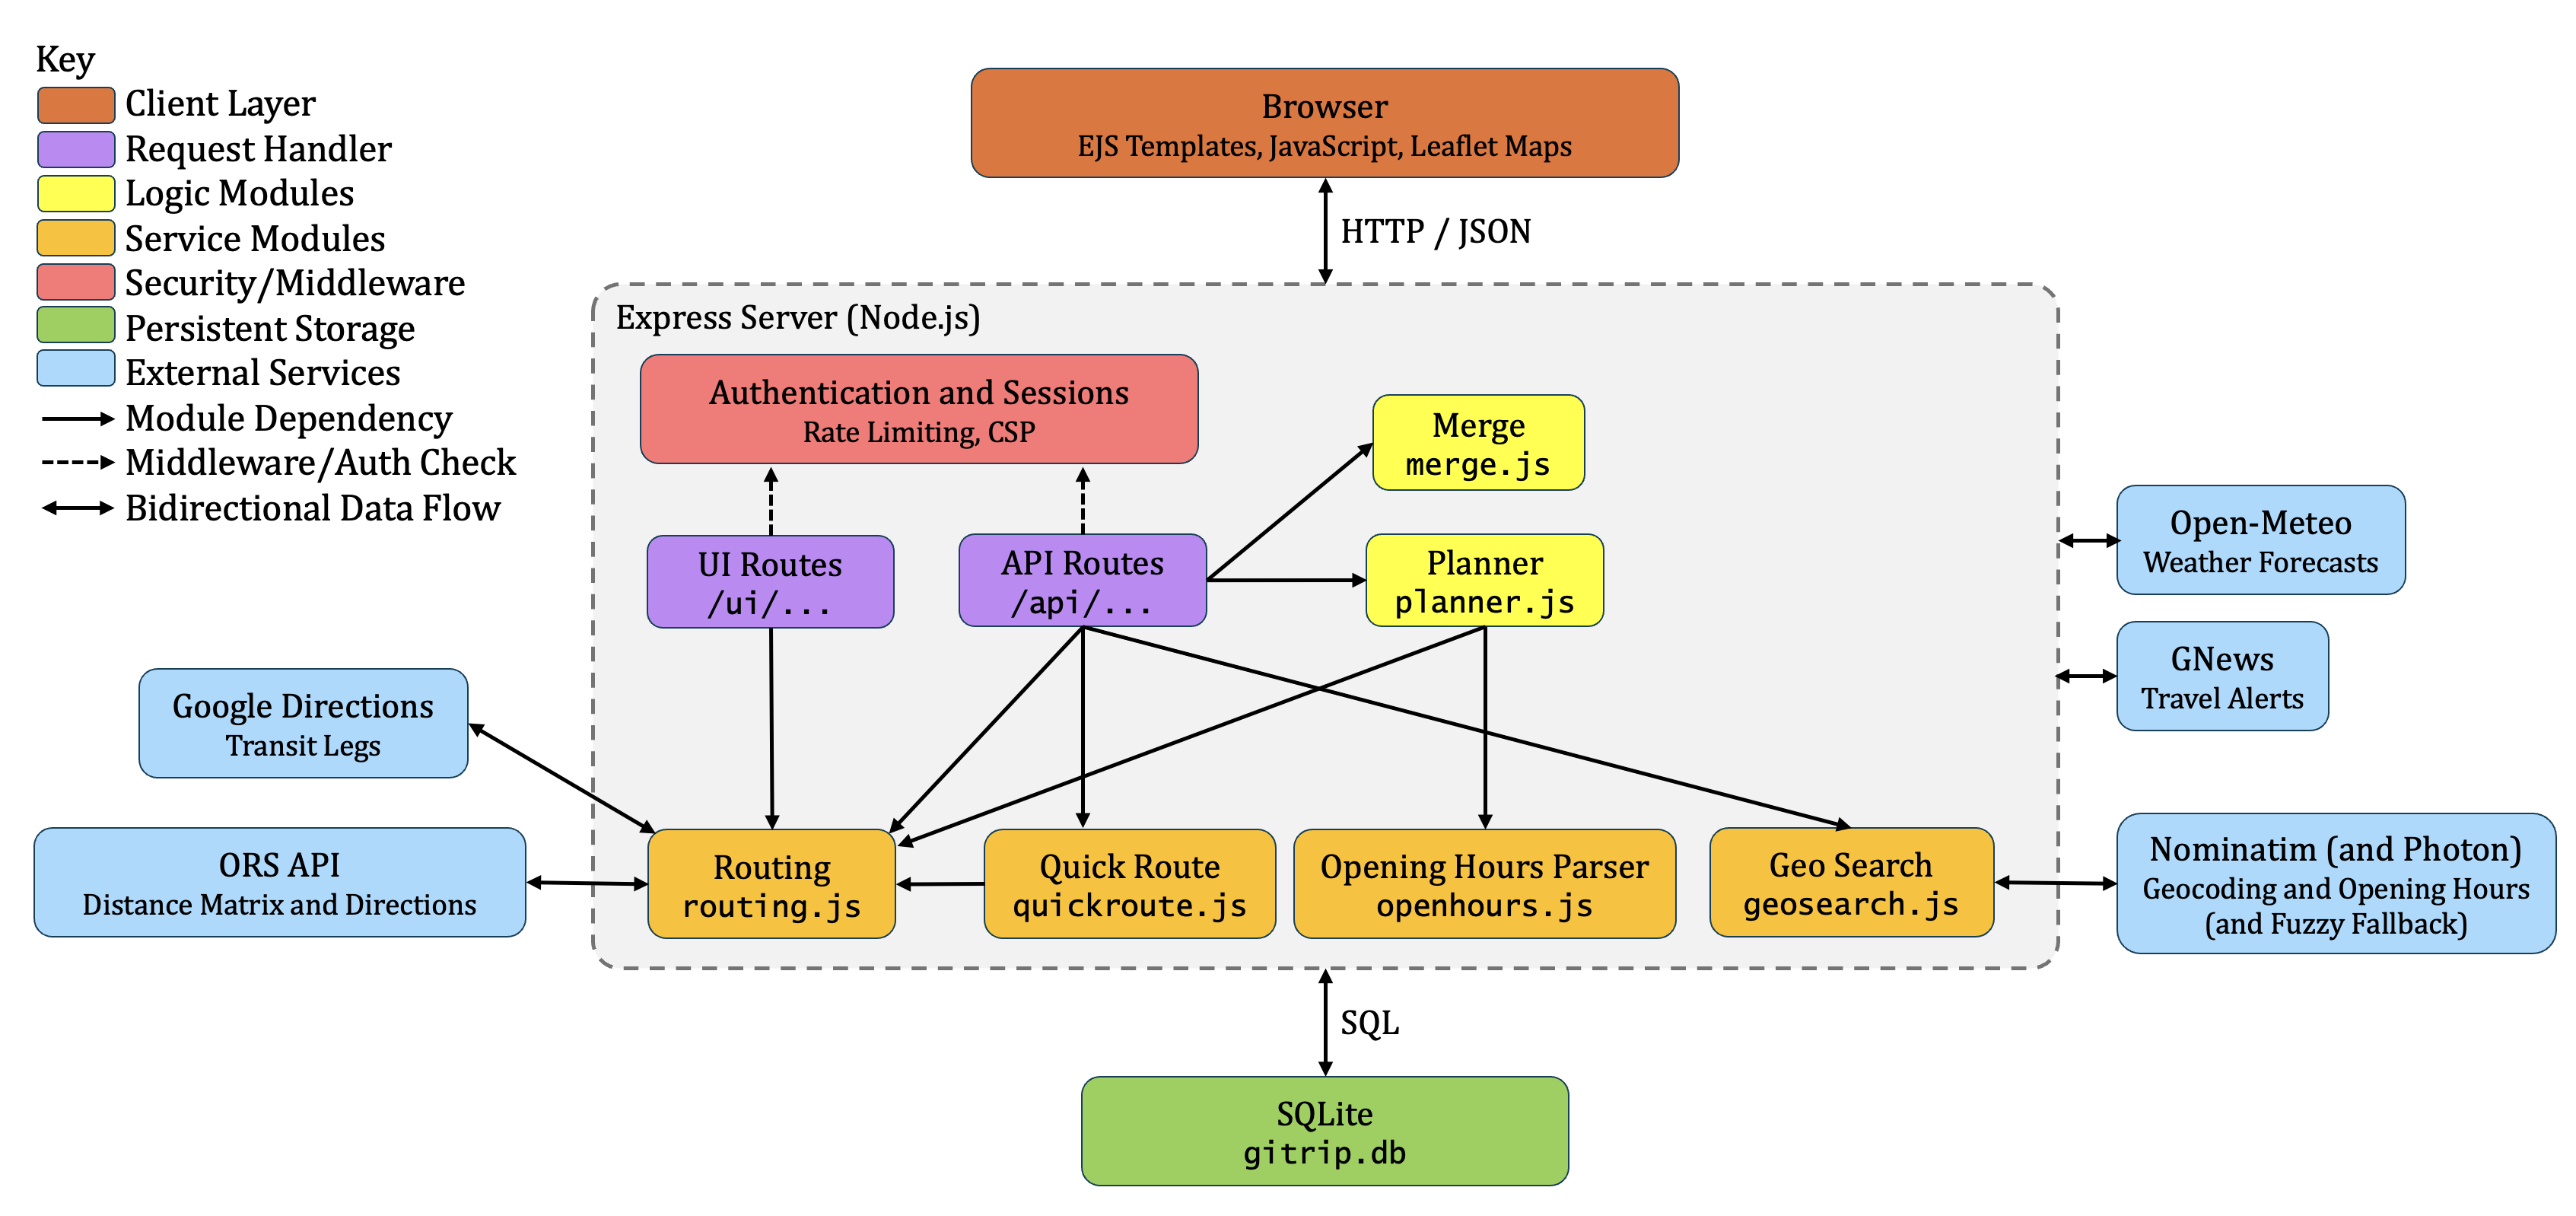
\includegraphics[width=\textwidth]{Chapter5/architecture-diagram.png}
  \caption{High-level system architecture of GiTrip.}
  \label{fig:architecture}
\end{figure}

\section{Data Model and Repository Semantics}
GiTrip's database schema includes the following core tables:
\begin{itemize}
  \item \textbf{repos:} repository metadata (title, owner, visibility, current
        branch, fork source), keyed by a Universally Unique Identifier (UUID).
  \item \textbf{branches:} named pointers to commits (head commit).
  \item \textbf{commits:} commit metadata and full snapshot storage.
        Each commit records its parent commit(s), forming a Directed Acyclic
        Graph (DAG) that represents the repository's version history.
\end{itemize}

Additional tables support authentication (\textbf{users}, \textbf{sessions}) and
social/collaboration (\textbf{repo\_collaborators}, \textbf{repo\_stars}).
Supporting planning features are stored in \textbf{travel\_alerts} and
\textbf{packing\_checklists}. Database indexes are defined on all foreign-key
columns (e.g., \texttt{commits.repo\_id}, \texttt{branches.repo\_id},
\texttt{repo\_stars.repo\_id}) to ensure query performance scales with data
growth.

Figure~\ref{fig:erd} shows the entity relationship (ER) diagram for GiTrip's data
model using Crow's foot notation. The core version-control triad (Repo, Branch, Commit) mirrors Git
semantics, while the embedded Snapshot structure captures itinerary-specific data
as JSON within each commit row. Solid-bordered entities are persisted as SQLite tables; dashed-bordered entities represent JSON structures embedded within the \texttt{snapshot} column of each Commit. Primary keys are underlined in the diagram. Crow's foot endpoints: double bar = exactly one, circle--bar = zero or one, fork--bar = one or many, fork--circle = zero or many.

\begin{figure}[H]
  \centering
  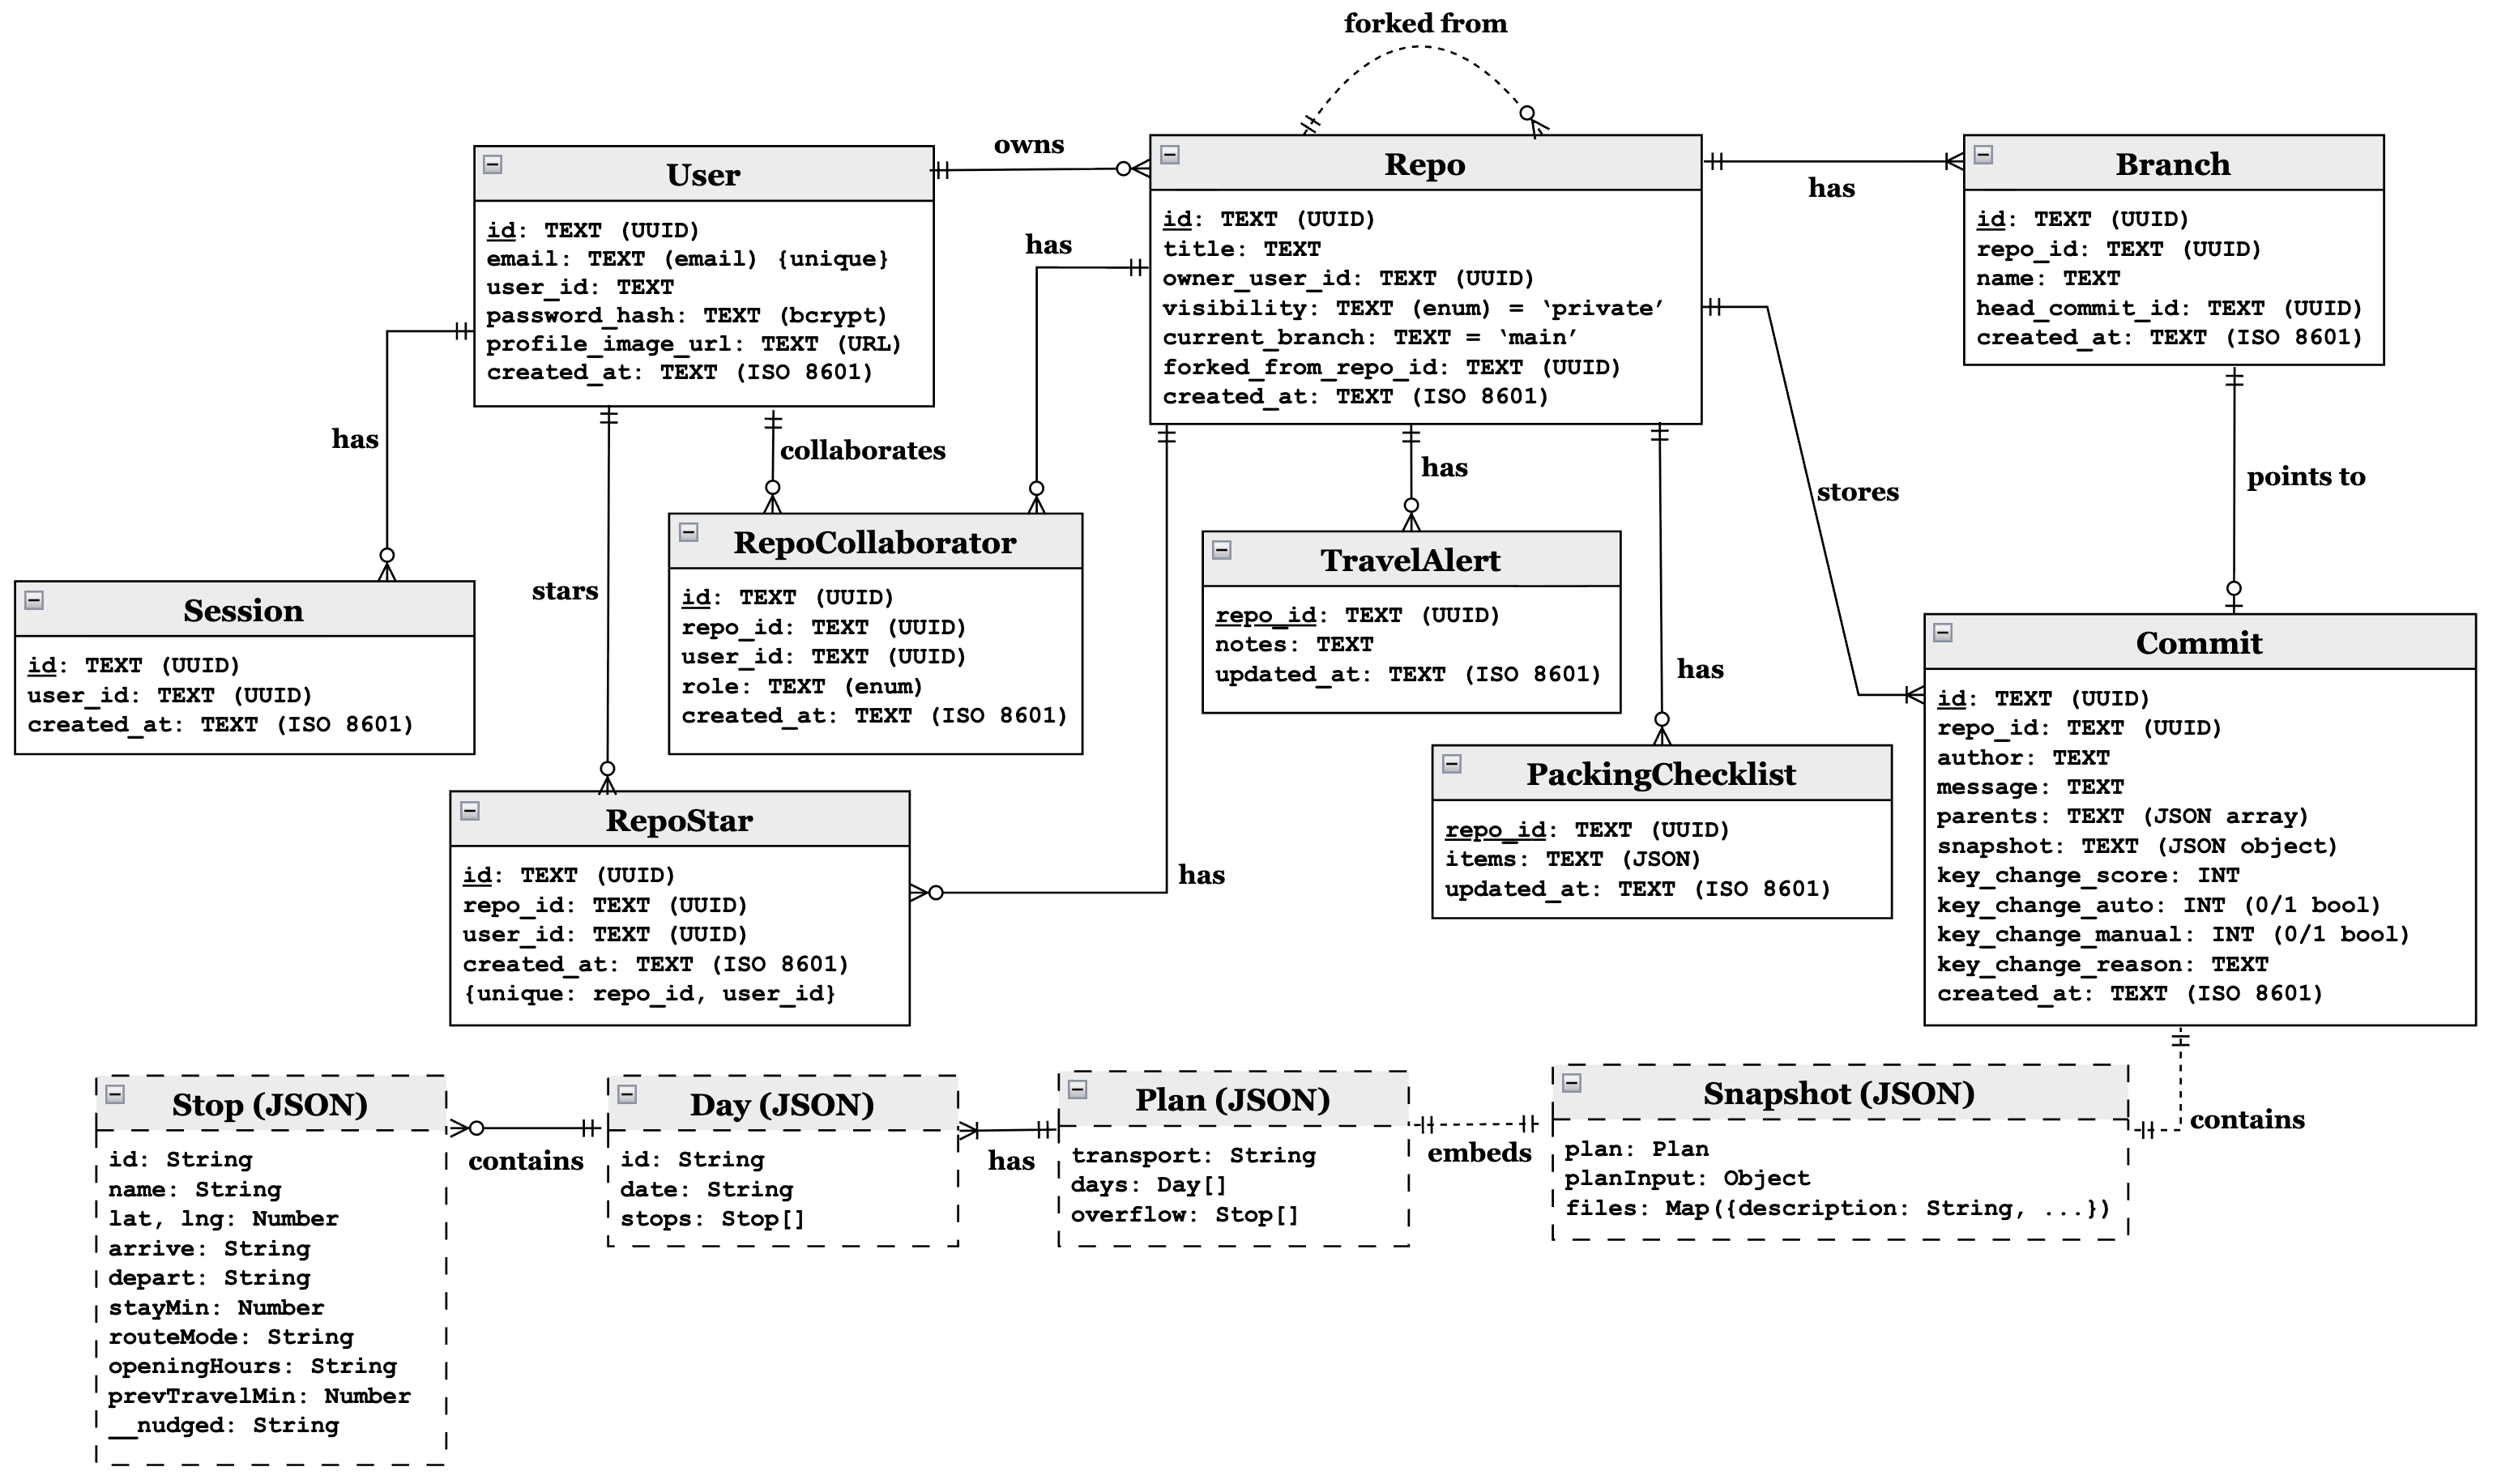
\includegraphics[width=\textwidth]{Chapter5/ER-diagram.png}
  \caption{Entity relationship diagram for GiTrip's data model.}
  \label{fig:erd}
\end{figure}

\subsection{Snapshot Storage}
Commits store complete plan snapshots. Snapshot versioning was selected over delta storage (method to store only the differences between versions) because it (i) simplifies branch switching and rollback (no delta replay), (ii) simplifies three-way merge (each tip contains a complete state), and (iii) remains feasible for the expected scale~\cite{ref_progit_snapshots}. Delta compression is noted as future work for production-scale repositories. Each snapshot contains:
\begin{itemize}
  \item \texttt{snapshot.plan}: the itinerary (days and stops).
  \item \texttt{snapshot.planInput}: planner inputs for reproducibility and UI defaults.
  \item \texttt{snapshot.files}: a key-value map for branch-level metadata. For example, the trip description (\texttt{files.description}), which collaborators can edit independently on separate branches. The merge engine performs per-key three-way merging on this map, detecting conflicts when both sides change the same key.
\end{itemize}

\subsection{Plan Schema}
A plan includes:
\begin{itemize}
  \item \texttt{transport} mode (driving/walking/cycling/transit),
  \item \texttt{days[]} each with \texttt{id}, \texttt{date}, and
        \texttt{stops[]},
  \item each stop includes identity, location, scheduling, and routing metadata.
\end{itemize}

Stops also carry planner constraint fields such as strict ordering, time windows,
fixed-time flags, and opening-hours strings. A \texttt{\_\_nudged} marker records
explainable adjustments made by the scheduler (e.g., nudged due to opening
hours).

\subsection{Module Structure}
Figure~\ref{fig:uml_class} shows the Unified Modeling Language (UML) class diagram for GiTrip's server-side
modules. Each module is represented as a class with its exported functions as
public operations (\texttt{+}) and internal helper functions as private
operations (\texttt{-}). The \texttt{Server} module acts as the central
orchestrator, delegating to specialised modules for planning, merging, routing,
and geocoding. \texttt{TTLCache} is the only formal JavaScript class in the
codebase; all other modules use the CommonJS \texttt{module.exports} pattern. In the diagram, dashed open arrows denote $\langle\!\langle$use$\rangle\!\rangle$ dependencies and the filled diamond denotes composition (Server owns TTLCache instances).

\begin{figure}[H]
  \centering
  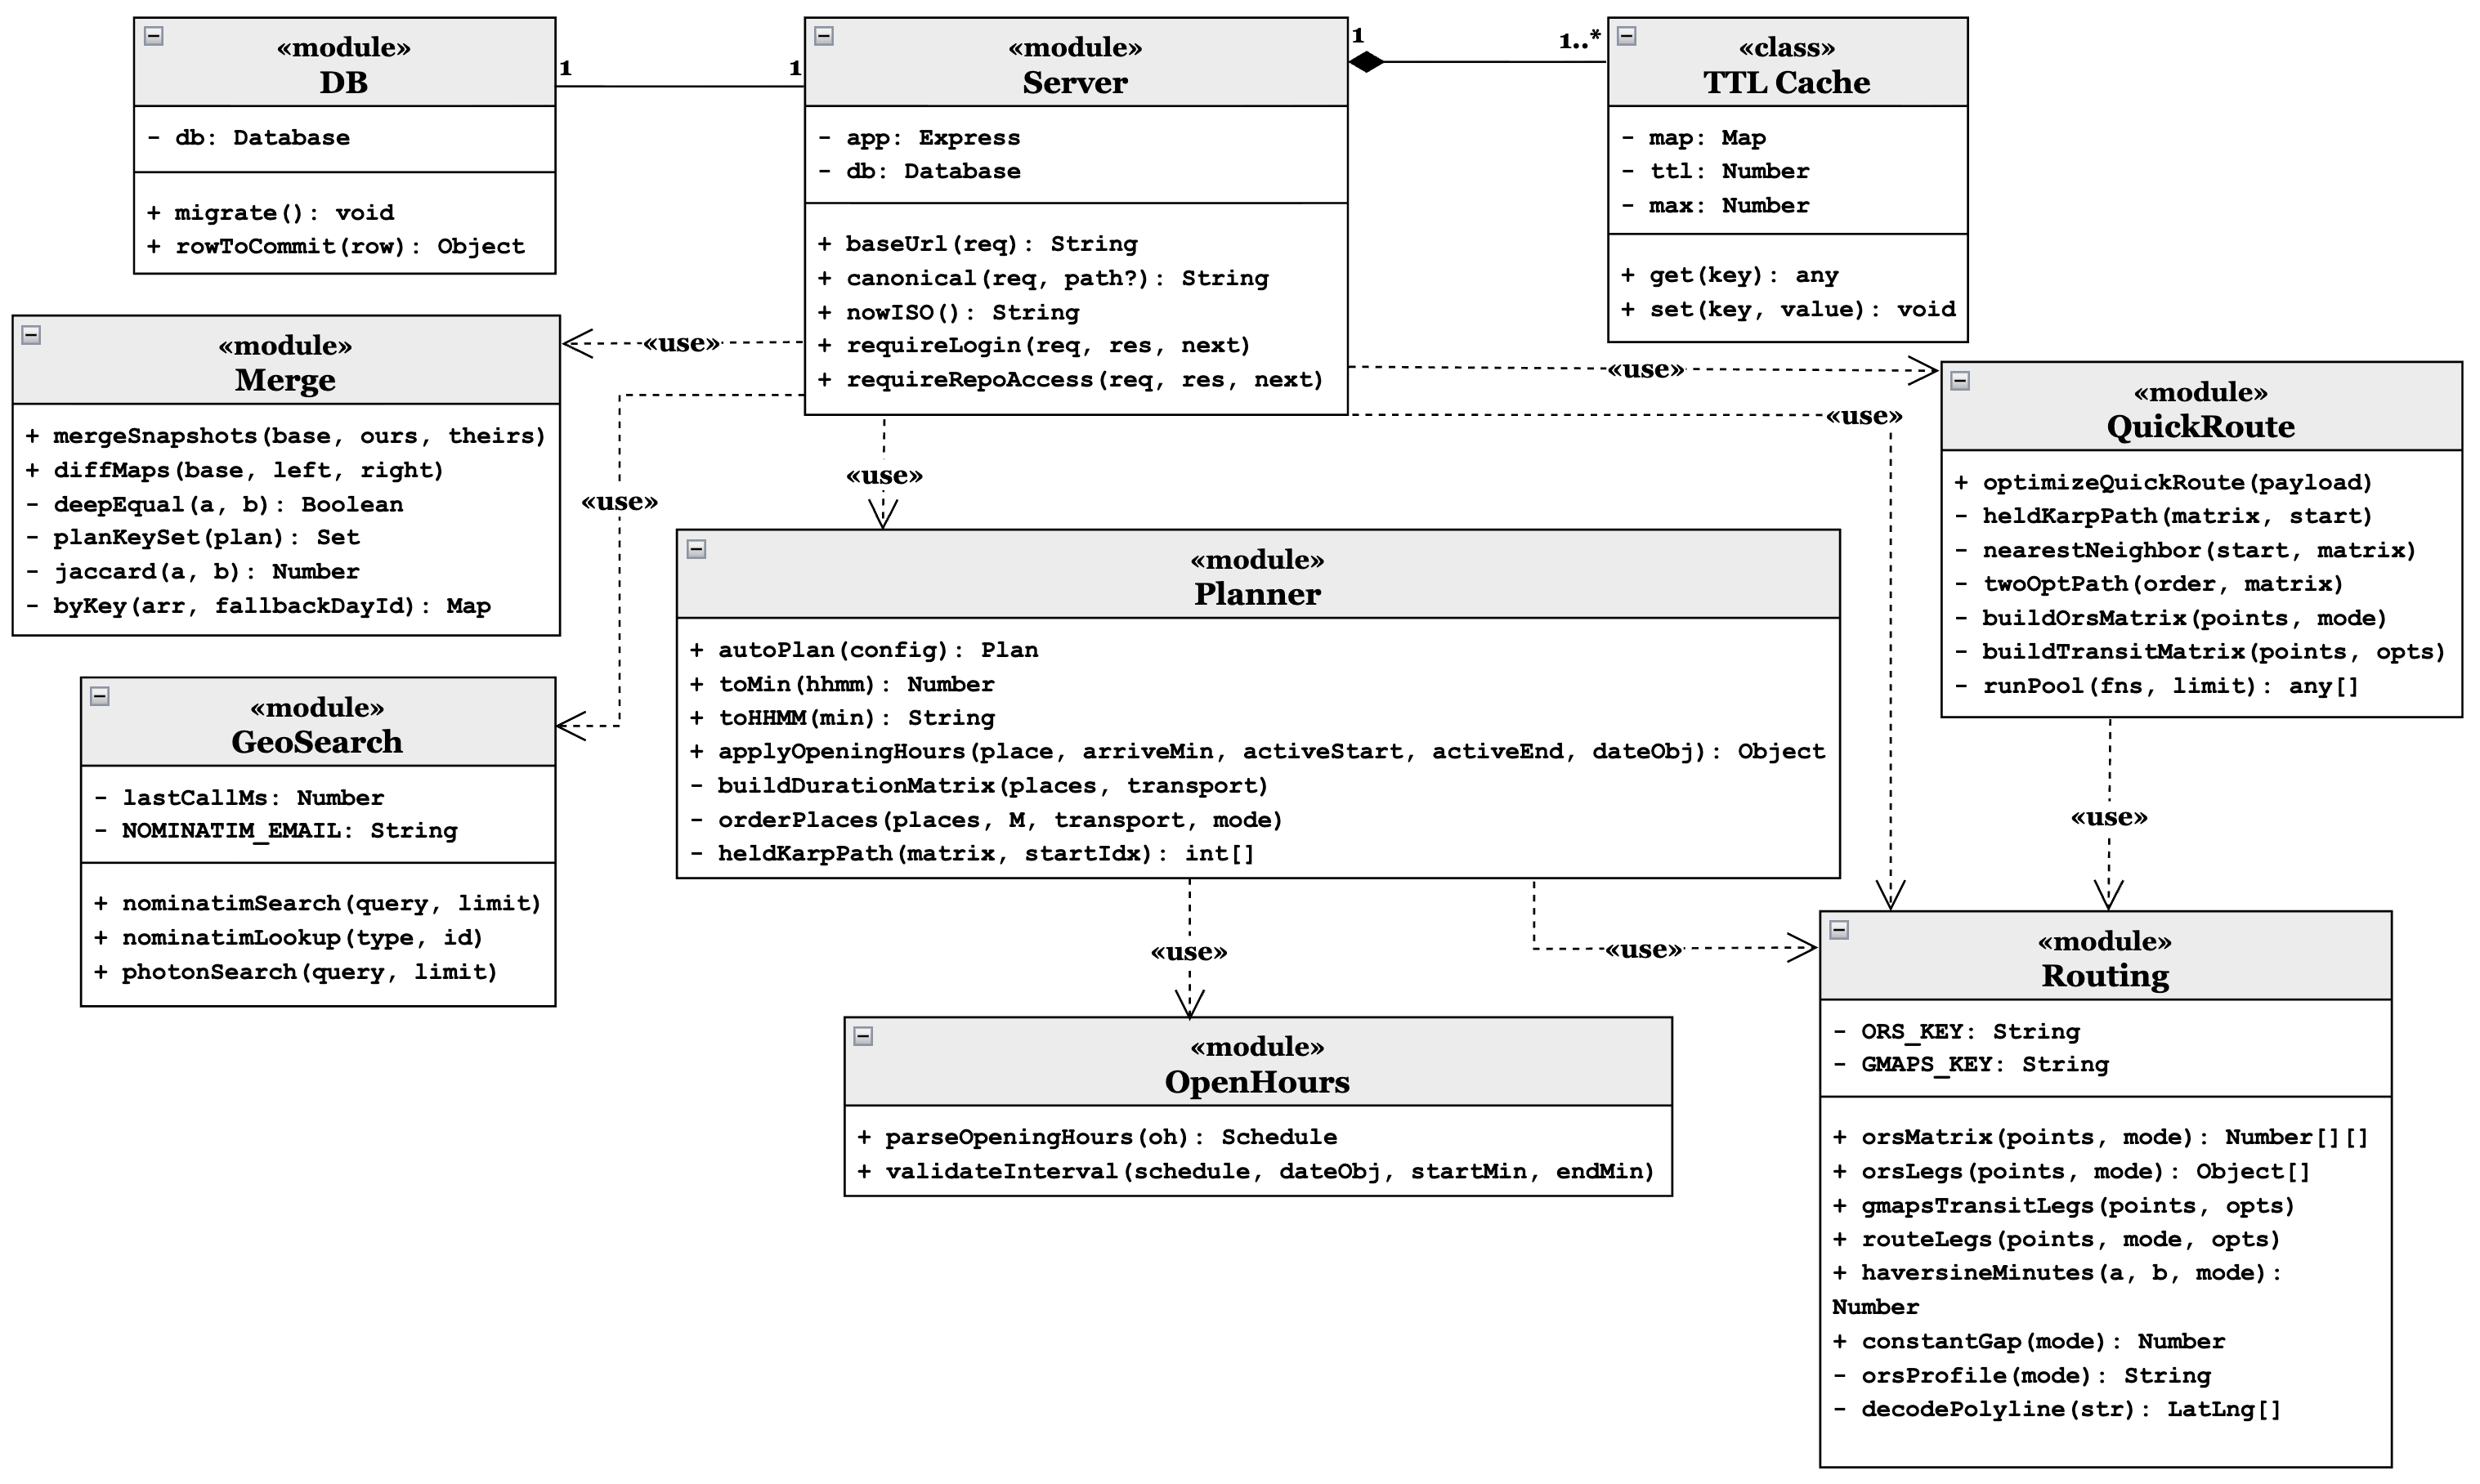
\includegraphics[width=\textwidth]{Chapter5/uml-class-diagram.png}
  \caption{UML class diagram for GiTrip's server-side modules.}
  \label{fig:uml_class}
\end{figure}

\section{Routing and Geocoding Design}
\subsection{Place Search}
GiTrip proxies Nominatim~\cite{ref_nominatim} search/lookup via server endpoints to enable caching and rate limiting. Results are re-ranked using approximate string matching to prioritise substring matches and reduce diacritic/punctuation sensitivity \cite{ref_navaro_string_matching}. Since Nominatim performs exact matching against its index, near-miss queries (e.g.\ ``stick n sushi'' for ``Sticks'n'Sushi'') can return zero results. To address this, GiTrip falls back to Photon~\cite{ref_photon} when Nominatim returns no matches. Photon is an open-source geocoder built on Elasticsearch that indexes the same OpenStreetMap data with n-gram tokenisation and typo tolerance, providing fuzzy search without requiring a separate dataset. The fallback is transparent: Photon results are returned in the same shape, with \texttt{opening\_hours} set to null since Photon does not expose that field.

\subsection{Routing Providers and Fallback}
Routing serves two purposes. First, ORS matrix endpoints compute pairwise travel durations for route ordering (driving/cycling/walking). The matrix endpoint reduces API calls from $O(n^2)$ pairwise requests to a single request per optimisation run. Second, per-leg routing provides geometries for map visualisation; Google Directions is used for transit legs, including decoding polylines and extracting step-level sub-modes to distinguish walking approach segments.

For non-transit modes, GiTrip requests a travel-time matrix from OpenRouteService~\cite{ref_ors_matrix}. For transit, GiTrip uses Google Directions API~\cite{ref_google_directions_api} for
sequential legs. When providers fail or are
unavailable, GiTrip falls back to Haversine-based time estimates (computing approximate travel duration from straight-line distance with mode-dependent speed assumptions) for ordering, and constant default travel gaps per mode (e.g., 15 minutes for driving, 30 minutes for transit) as a safety margin when no routing data is available at all. This design ensures the planner remains usable even in degraded conditions, which is important for evaluation environments and offline/limited-connectivity contexts.

\section{Auto-scheduler Design}
The scheduler must construct a feasible plan that respects constraints. GiTrip's
scheduler is designed around four stages:
\begin{enumerate}
  \item \textbf{Matrix construction:} request pairwise travel durations (when
        available).
  \item \textbf{Ordering:} determine visit order using strict order constraints
        when provided; otherwise use Held-Karp exact solver for small instances
        ($N \leq 12$) \cite{ref_tsp_study} or Nearest Neighbour with 2-Opt
        refinement for larger instances
        \cite{ref_nn_tsp,ref_nn_2opt_hybrid}.
  \item \textbf{Packing into days:} greedily place stops into day windows while
        maintaining non-overlap and travel gaps.
  \item \textbf{Constraint enforcement:} apply opening hours, desired windows,
        and fixed-time constraints; if a stop cannot fit, spill it to a
        subsequent day or overflow.
\end{enumerate}

Given ordered stops $S_1,\dots,S_n$, per-leg travel $T_i$ (minutes from $S_{i-1}$ to $S_i$), stay durations $D_i$, active window $[A,B]$, break $b$, and focus offset $f$:
\[
a_1 = A+f,\quad d_1=a_1+D_1,\quad
a_i = d_{i-1}+b+T_i,\quad d_i=a_i+D_i \ (i>1).
\]
If $(a_i,d_i)$ violates a desired window or opening-hours constraint, the scheduler shifts to the nearest valid interval inside $[A,B]$; otherwise, it spills to the next day's $A+f$. The user preference (compact vs.\ sparse) controls additional free time after each stop.

\subsection{Opening Hours Nudging}
Opening hours are treated as a hard-ish constraint: if the proposed interval
falls in a closed period, the scheduler nudges to the next open slot where
feasible; otherwise the stop is rejected for that day. This is crucial for
feasibility and directly addresses common itinerary failures in real planning.

\subsection{Compact vs Sparse Modes}
To improve user control over schedule density, the scheduler supports
``compact'' and ``sparse'' modes. Compact mode packs stops tightly, while sparse
mode distributes stops across the active window by inserting additional gap time.
This preference improves perceived usefulness because different trip styles (e.g.,
city sprint vs relaxed exploration) require different pacing.

\subsection{Design Trade-offs and Pseudocode}
A key design trade-off in the scheduler is the choice of NN ordering over more sophisticated approaches such as exact TSP solvers~\cite{ref_tsp_study} or meta-heuristics~\cite{ref_tsp_local_search}. NN was selected because: (i) it runs in $O(n^2)$ time and performs acceptably for typical trip sizes ($n \le 50$ stops), (ii) it avoids the implementation complexity and computational cost of exact solvers, and (iii) API quota constraints make it infeasible to request large distance matrices repeatedly during interactive editing. For trips with more than 50 stops, the scheduler divides the itinerary into day-sized chunks and optimises each independently, which maintains reasonable performance while accepting some suboptimality in cross-day transitions. The full pseudocode for the auto-scheduler is presented in Chapter~\ref{ch:implementation} (Algorithm~\ref{alg:planner}).

\section{Merge Design}
GiTrip implements a Git-style three-way merge for snapshots. The merge process
uses:
\begin{itemize}
  \item a \textbf{base} snapshot, the lowest common ancestor (LCA),
  \item \textbf{ours} and \textbf{theirs} snapshots (branch heads),
  \item a merge engine producing a merged snapshot plus a list of conflicts.
\end{itemize}

The fundamental principle, inherited from Git's merge model, is that a conflict
only arises when \textbf{both} branches express a different opinion about the
same data relative to the base. If only one branch changes a stop (or deletes
it) and the other leaves it untouched, the merge engine cleanly accepts the
change---just as \texttt{git merge} auto-resolves one-sided edits. For example,
if one branch deletes a stop and the other never touched it, the deletion is
accepted; a conflict is raised only if the other branch also \textit{edited}
that stop, creating a genuine disagreement.

Figure~\ref{fig:merge_flow} illustrates the full decision logic of the merge
engine. The engine first iterates all file keys, recording conflicts or taking the changed side, then checks plan divergence. If both sides changed the plan identically, either is taken. If both changed the plan structure and their stop-key Jaccard similarity is below~0.4, a whole-plan conflict is raised. Otherwise, per-stop merging chains through deletion, time, and field checks. The result is stabilised by deterministic ordering before output.

\begin{figure}[H]
  \centering
  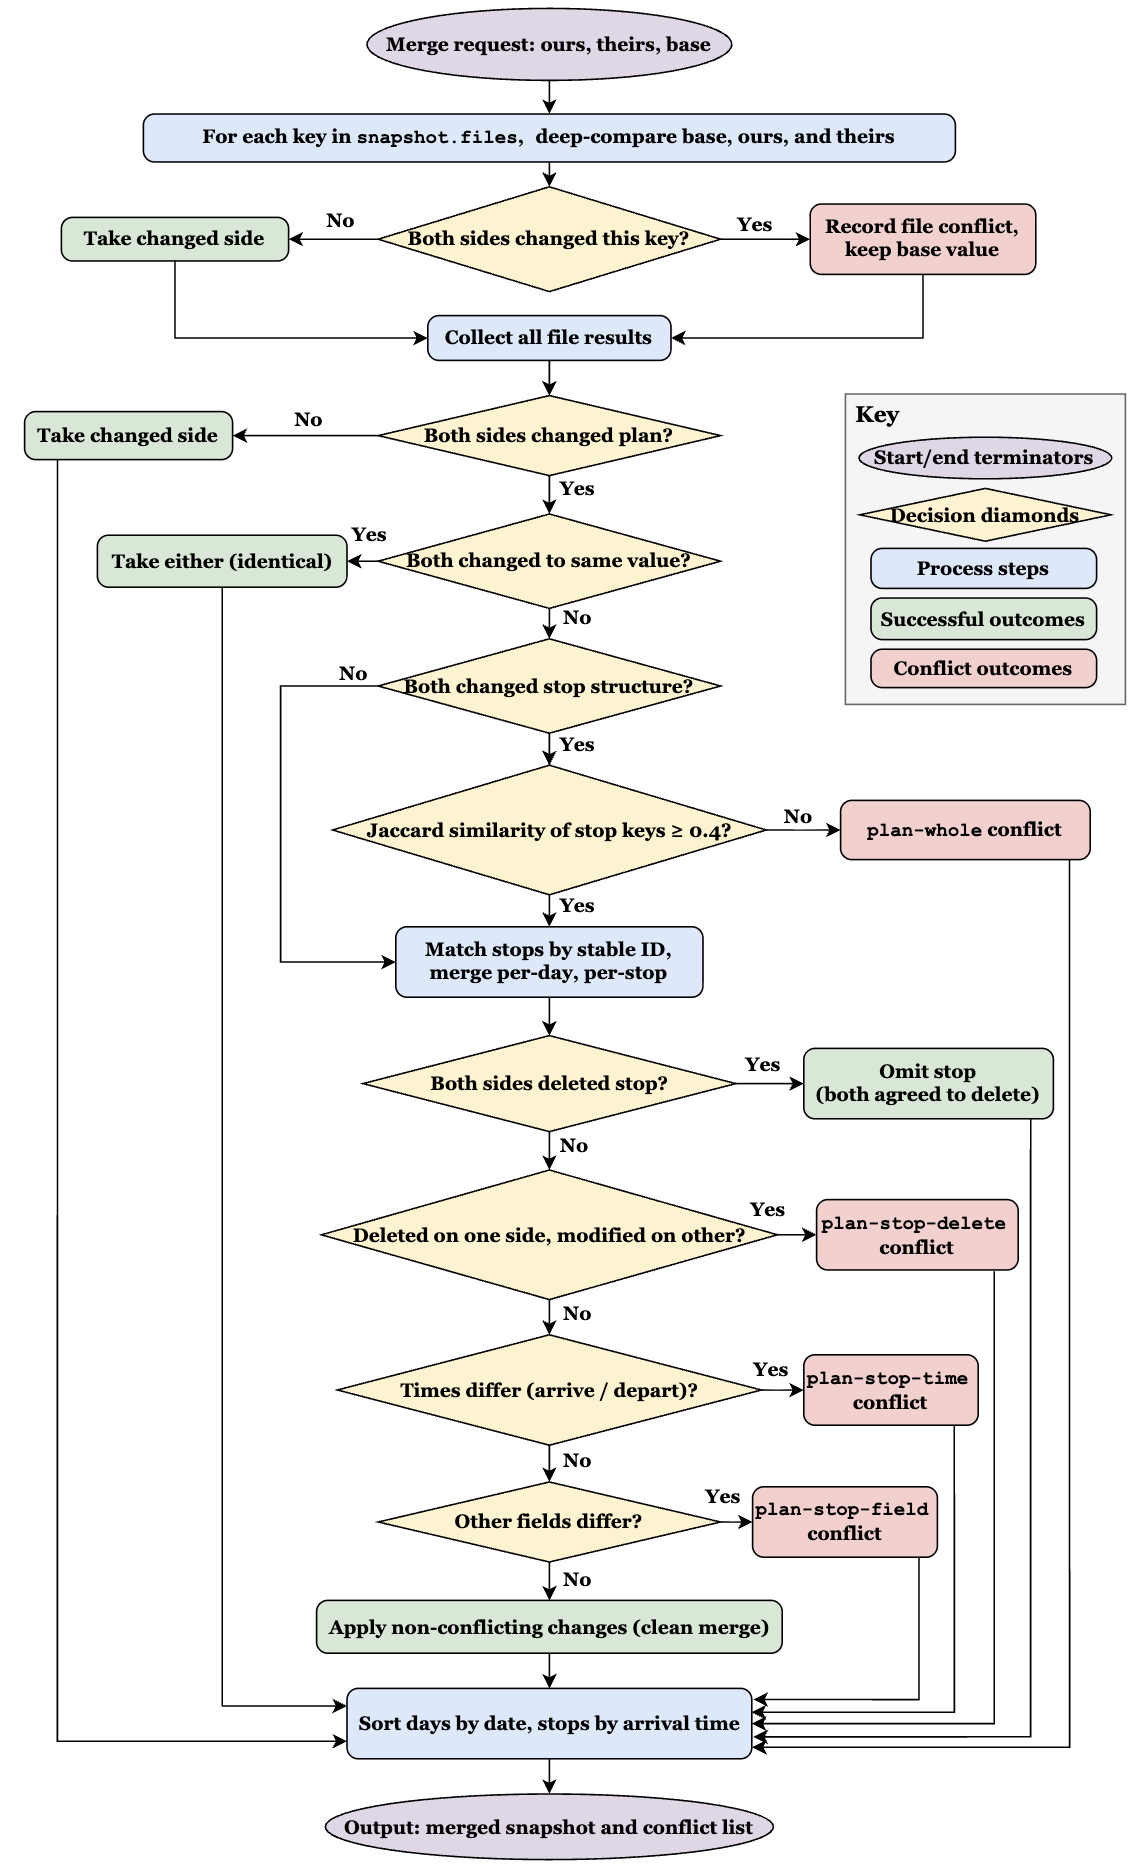
\includegraphics[width=0.9\textwidth]{Chapter5/merge-flowchart.png}
  \caption{Three-way merge decision flowchart.}
  \label{fig:merge_flow}
\end{figure}

\subsection{Equality and Stability}
Early merge implementations that relied on \texttt{JSON.stringify} can be brittle
because key insertion order may differ and \texttt{undefined} values are dropped.
The final implementation uses deep structural equality, making comparisons
key-order independent.

Additionally, merged ordering is stabilised by sorting days by ISO date and
sorting stops by arrival time (then name). This reduces surprising reordering
after merges.

\subsection{Conflict Types}
Conflicts surfaced include:
\begin{itemize}
  \item \textbf{file:} both sides changed the same key in \texttt{snapshot.files} (e.g., the trip description).
  \item \textbf{plan-stop-time:} both sides changed arrival/departure times
        differently for the same stop.
  \item \textbf{plan-stop-delete:} one side deleted a stop while the other
        modified it.
  \item \textbf{plan-stop-field:} times agree but both sides changed selected
        fields differently (e.g., name, lat/lng, notes, stayMin, routeMode).
  \item \textbf{plan-whole:} plans diverged heavily (Jaccard similarity of
        stop-key sets below 0.4), requiring whole-plan selection.
\end{itemize}

This set is intentionally constrained to keep the UI manageable for non-experts
while still preventing silent data loss.

\section{User Interface Design}
GiTrip uses server-rendered pages enhanced by client-side JavaScript. Two
interactive surfaces support editing:
\begin{itemize}
  \item \textbf{Timeline editor:} draggable blocks and handles adjust
        arrival/departure times with snapping and constraint clamping.
  \item \textbf{Map editor:} draggable numbered markers adjust stop coordinates
        and update route geometry.
\end{itemize}

\subsection{Easy Mode vs Git Mode}
In Q8 of the survey, asking if there are any concerns with this project, 6/11 respondents mentioned that \textit{Git} concept may be complicated for users without a technical background. To reduce this cognitive overhead while preserving versioning power for advanced users, the ``Git mode'' toggle button was invented. When turned off, the UI replaces \textit{Git}-related terminologies with task-oriented wording (e.g., ``Save trip'' rather than ``Commit''), while keeping the functionality same. In addition, when turned off, the advanced auto-scheduler workflow is complemented by an easy-mode scheduling path (Appendix~\ref{appx:diagrams}), where users can create a trip by entering a bullet-point stop list and letting the system generate and commit a feasible itinerary. This design keeps the novice workflow ``single-track'' (plan $\rightarrow$ save $\rightarrow$ refine) while allowing expert users to opt into full version-control semantics without losing compatibility with the stored data.

GiTrip therefore includes a mode toggle:
\begin{itemize}
  \item \textbf{Easy mode:} hides branches/commits/merge; offers ``Save trip''
        with non-fast-forward friendly behaviour.
  \item \textbf{Git mode:} exposes full repository semantics and merge UI.
\end{itemize}

This design supports two user personas without splitting the product into
separate applications.

\subsection{Quick Explore Mode}
The ``Quick route'' page adopts a \textit{Google Maps}-like interaction style to minimise onboarding friction: the primary surface is a map plus a simple stop list, and the user can immediately compute an optimised order and per-leg travel times without first understanding repositories, branches, or commits. This design matches a common mental model for trip planning (enter places $\rightarrow$ see route $\rightarrow$ iterate), and it also includes a bookmark feature that lets users save places and immediately compute the entire route when pressed. Crucially, \textit{GiTrip} connects this streamlined workflow back to the full versioned system via ``Save as Repository'': once the user is satisfied with a route, the system creates a repository and an initial snapshot commit containing the generated plan. This provides a low-friction entry point for new users, while still enabling the richer repository workflow (timeline editing, map refinement, branching, and merging) when needed.

\section{Security, Privacy, and Accessibility Design}
GiTrip includes several practical web security measures:
\begin{itemize}
  \item session cookies are HttpOnly and SameSite=Lax,
  \item security headers include CSP, frame blocking, and HTTP Strict Transport Security (HSTS) in production,
  \item rate limiting is applied globally and more strictly on sensitive
        endpoints (four tiers: global, API, geo search, and authentication),
  \item prepared statements are used for SQLite queries to reduce SQL injection
        risk,
  \item error responses return generic messages to users while logging full
        details server-side, preventing information leakage of internal paths
        or stack traces.
\end{itemize}

Accessibility is guided by WCAG 2.2~\cite{ref_wcag22}. The UI uses labelled
controls and avoids information conveyed only by colour; however, interactive
map/timeline controls remain a known accessibility challenge and are discussed as
a limitation.

% !TEX root = ../Report.tex
% ======================================================================
\chapter{Implementation}
\label{ch:implementation}
% ======================================================================

This chapter documents how the design was realised in code, covering major
implementation modules and the reasoning behind key decisions.

\section{Backend Structure}
The backend is a Node.js and Express application \cite{ref_node_about,ref_express}.
The main server file configures:
\begin{itemize}
  \item EJS templating for UI routes,
  \item JSON body limits for planner payloads,
  \item authentication sessions (\texttt{gitrip\_sid}),
  \item security headers and rate limiting,
  \item caching for external API calls (geocoding and weather).
\end{itemize}

\subsection{Database Layer}
The database layer uses \texttt{better-sqlite3} and maintains schema migrations
in a single module. Commit rows store JSON fields (\texttt{parents},
\texttt{snapshot}) as strings and are deserialised on load. The schema
intentionally does not enforce foreign keys at the SQLite level; relationships
are handled logically by the application. Indexes are created on all
foreign-key columns (e.g., \texttt{commits.repo\_id},
\texttt{branches.repo\_id}, \texttt{repo\_stars.repo\_id/user\_id}) to
maintain query performance as the number of repositories and commits grows.

\subsection{Error Handling}
All error responses sent to users use generic messages (e.g., ``Planner error.
Please try again.'') rather than exposing internal error details. Full error
information is logged server-side via \texttt{console.error} for debugging.
This prevents information leakage of internal paths, stack traces, or
dependency details that could aid reconnaissance.

\section{Planner Implementation}
\label{sec:planner-impl}
The auto-scheduler is implemented in \texttt{server/planner.js}. Key components
include:
\begin{itemize}
  \item \textbf{Time helpers:} \texttt{toMin} and \texttt{toHHMM}.
  \item \textbf{Matrix building:} ORS matrix for non-transit; null for transit.
  \item \textbf{Ordering logic:} strict order handling (absolute or relative);
        when no strict orders exist, Held-Karp exact solver for $N \leq 12$
        \cite{ref_tsp_study}, otherwise Nearest Neighbour with 2-Opt refinement
        \cite{ref_nn_tsp,ref_nn_2opt_hybrid}.
  \item \textbf{Constraint fit check:} \texttt{applyOpeningHours} integrates
        active hours, desired windows, fixed-time behaviour, and opening-hours
        nudging.
  \item \textbf{Packing loop:} schedules preferred-day buckets first, then
        unassigned stops, spilling to later days or overflow when necessary.
\end{itemize}

The planner records travel minutes (\texttt{prevTravelMin}) and effective route
mode per leg, including detection of transit vs walking in cases where the
transit provider returns walking-only legs.

The ordering stage uses three strategies depending on instance size, presented in Algorithms~\ref{alg:nn}--\ref{alg:heldkarp}. The NN heuristic (Algorithm~\ref{alg:nn}) greedily selects the closest unvisited stop; if no finite edge exists from the current node, remaining stops are appended in their original input order. The 2-Opt refinement (Algorithm~\ref{alg:twoopt}) iteratively reverses sub-segments to reduce total cost, keeping the origin fixed and running up to 4 sweeps or until no improvement is found. The Held-Karp solver (Algorithm~\ref{alg:heldkarp}) solves for the shortest \emph{path} (open tour), not a cycle, unlike the classic TSP formulation.

\begin{algorithm}[H]
  \caption{Nearest Neighbour heuristic - greedy $O(N^2)$ path construction.}
  \label{alg:nn}
  \begin{algorithmic}[1]
    \Require travel-time matrix $M$, start index $s$
    \Ensure  visit order $\mathit{order}$
    \State $\mathit{order} \gets [s]$; \; $\mathit{used}[s] \gets \textbf{true}$
    \While{$|\mathit{order}| < N$}
      \State $\mathit{cur} \gets \mathit{order}.\mathrm{last}$
      \State $\mathit{best} \gets \arg\min_{j \notin \mathit{used}} M[\mathit{cur}][j]$
      \If{$\mathit{best}$ exists}
        \State $\mathit{used}[\mathit{best}] \gets \textbf{true}$; \;
               append $\mathit{best}$ to $\mathit{order}$
      \Else
        \State append all remaining unvisited nodes in original index order
        \State \textbf{break}
      \EndIf
    \EndWhile
    \State \Return $\mathit{order}$
  \end{algorithmic}
\end{algorithm}

\begin{algorithm}[H]
  \caption{2-Opt local search refinement.}
  \label{alg:twoopt}
  \begin{algorithmic}[1]
    \Require visit order $\mathit{order}$, travel-time matrix $M$
    \Ensure  improved visit order $\mathit{best}$
    \State $\mathit{best} \gets \mathit{order}$; \;
           $\mathit{bestCost} \gets \Call{PathCost}{\mathit{best}, M}$
    \For{$\mathit{pass} \gets 1$ \textbf{to} $4$}
      \State $\mathit{improved} \gets \textbf{false}$
      \For{$i \gets 1$ \textbf{to} $N - 3$}
        \Comment{skip index 0 to fix origin}
        \For{$k \gets i + 1$ \textbf{to} $N - 2$}
          \State $\mathit{cand} \gets \mathit{best}$ with segment $[i \ldots k]$ reversed
          \If{$\Call{PathCost}{\mathit{cand}, M} < \mathit{bestCost}$}
            \State $\mathit{best} \gets \mathit{cand}$; \;
                   $\mathit{bestCost} \gets \Call{PathCost}{\mathit{cand}, M}$; \;
                   $\mathit{improved} \gets \textbf{true}$
          \EndIf
        \EndFor
      \EndFor
      \If{$\lnot\mathit{improved}$} \textbf{break} \EndIf
    \EndFor
    \State \Return $\mathit{best}$
  \end{algorithmic}
\end{algorithm}

\begin{algorithm}[H]
  \caption{Held-Karp exact solver - bitmask DP in $O(2^N \cdot N^2)$, used for $N \leq 12$.}
  \label{alg:heldkarp}
  \begin{algorithmic}[1]
    \Require travel-time matrix $M$, start index $s$
    \Ensure  optimal visit order $\mathit{order}$, cost
    \State $N \gets |M|$; \; $\mathit{FULL} \gets 2^N - 1$
    \State $\mathit{dp}[\mathit{mask}][j] \gets \infty$ for all $(\mathit{mask}, j)$
    \State $\mathit{parent}[\mathit{mask}][j] \gets -1$ for all $(\mathit{mask}, j)$
    \State $\mathit{dp}[2^s][s] \gets 0$
      \Comment{base case: start at $s$}

    \Statex
    \For{$\mathit{mask} \gets 0$ \textbf{to} $\mathit{FULL}$}
      \If{bit $s$ not set in $\mathit{mask}$} \textbf{continue} \EndIf
      \For{$j \gets 0$ \textbf{to} $N-1$ where bit $j$ set in $\mathit{mask}$}
        \For{$k \gets 0$ \textbf{to} $N-1$ where bit $k$ \emph{not} set in $\mathit{mask}$}
          \State $\mathit{nm} \gets \mathit{mask} \;\mathbin{|}\; 2^k$
          \If{$\mathit{dp}[\mathit{mask}][j] + M[j][k] < \mathit{dp}[\mathit{nm}][k]$}
            \State $\mathit{dp}[\mathit{nm}][k] \gets \mathit{dp}[\mathit{mask}][j] + M[j][k]$
            \State $\mathit{parent}[\mathit{nm}][k] \gets j$
          \EndIf
        \EndFor
      \EndFor
    \EndFor

    \Statex \Comment{--- Reconstruct optimal path ---}
    \State $\mathit{bestEnd} \gets \arg\min_j \mathit{dp}[\mathit{FULL}][j]$
    \State $\mathit{order} \gets []$; \; $\mathit{mask} \gets \mathit{FULL}$; \;
           $\mathit{cur} \gets \mathit{bestEnd}$
    \While{$\mathit{cur} \neq -1$}
      \State prepend $\mathit{cur}$ to $\mathit{order}$
      \State $\mathit{prev} \gets \mathit{parent}[\mathit{mask}][\mathit{cur}]$; \;
             clear bit $\mathit{cur}$ from $\mathit{mask}$; \;
             $\mathit{cur} \gets \mathit{prev}$
    \EndWhile
    \State \Return $(\mathit{order},\;\mathit{dp}[\mathit{FULL}][\mathit{bestEnd}])$
  \end{algorithmic}
\end{algorithm}

Figure~\ref{fig:planner_flow} shows the auto-scheduler flowchart. The algorithm builds an ORS travel-time matrix (with Haversine fallback), orders stops (strict constraints, Held-Karp for $N \leq 12$, or NN and 2-Opt), then partitions them into preferred-day buckets and an unassigned pool. Phase~1 schedules preferred-day stops on their assigned day, sending unfitting stops directly to overflow. Phase~2 schedules unassigned stops greedily, spilling to subsequent days (retrying the same stop) or overflow when no days remain. The cursor is initialised with a focus-dependent shift (morning, midday, or afternoon).

\begin{figure}[H]
  \centering
  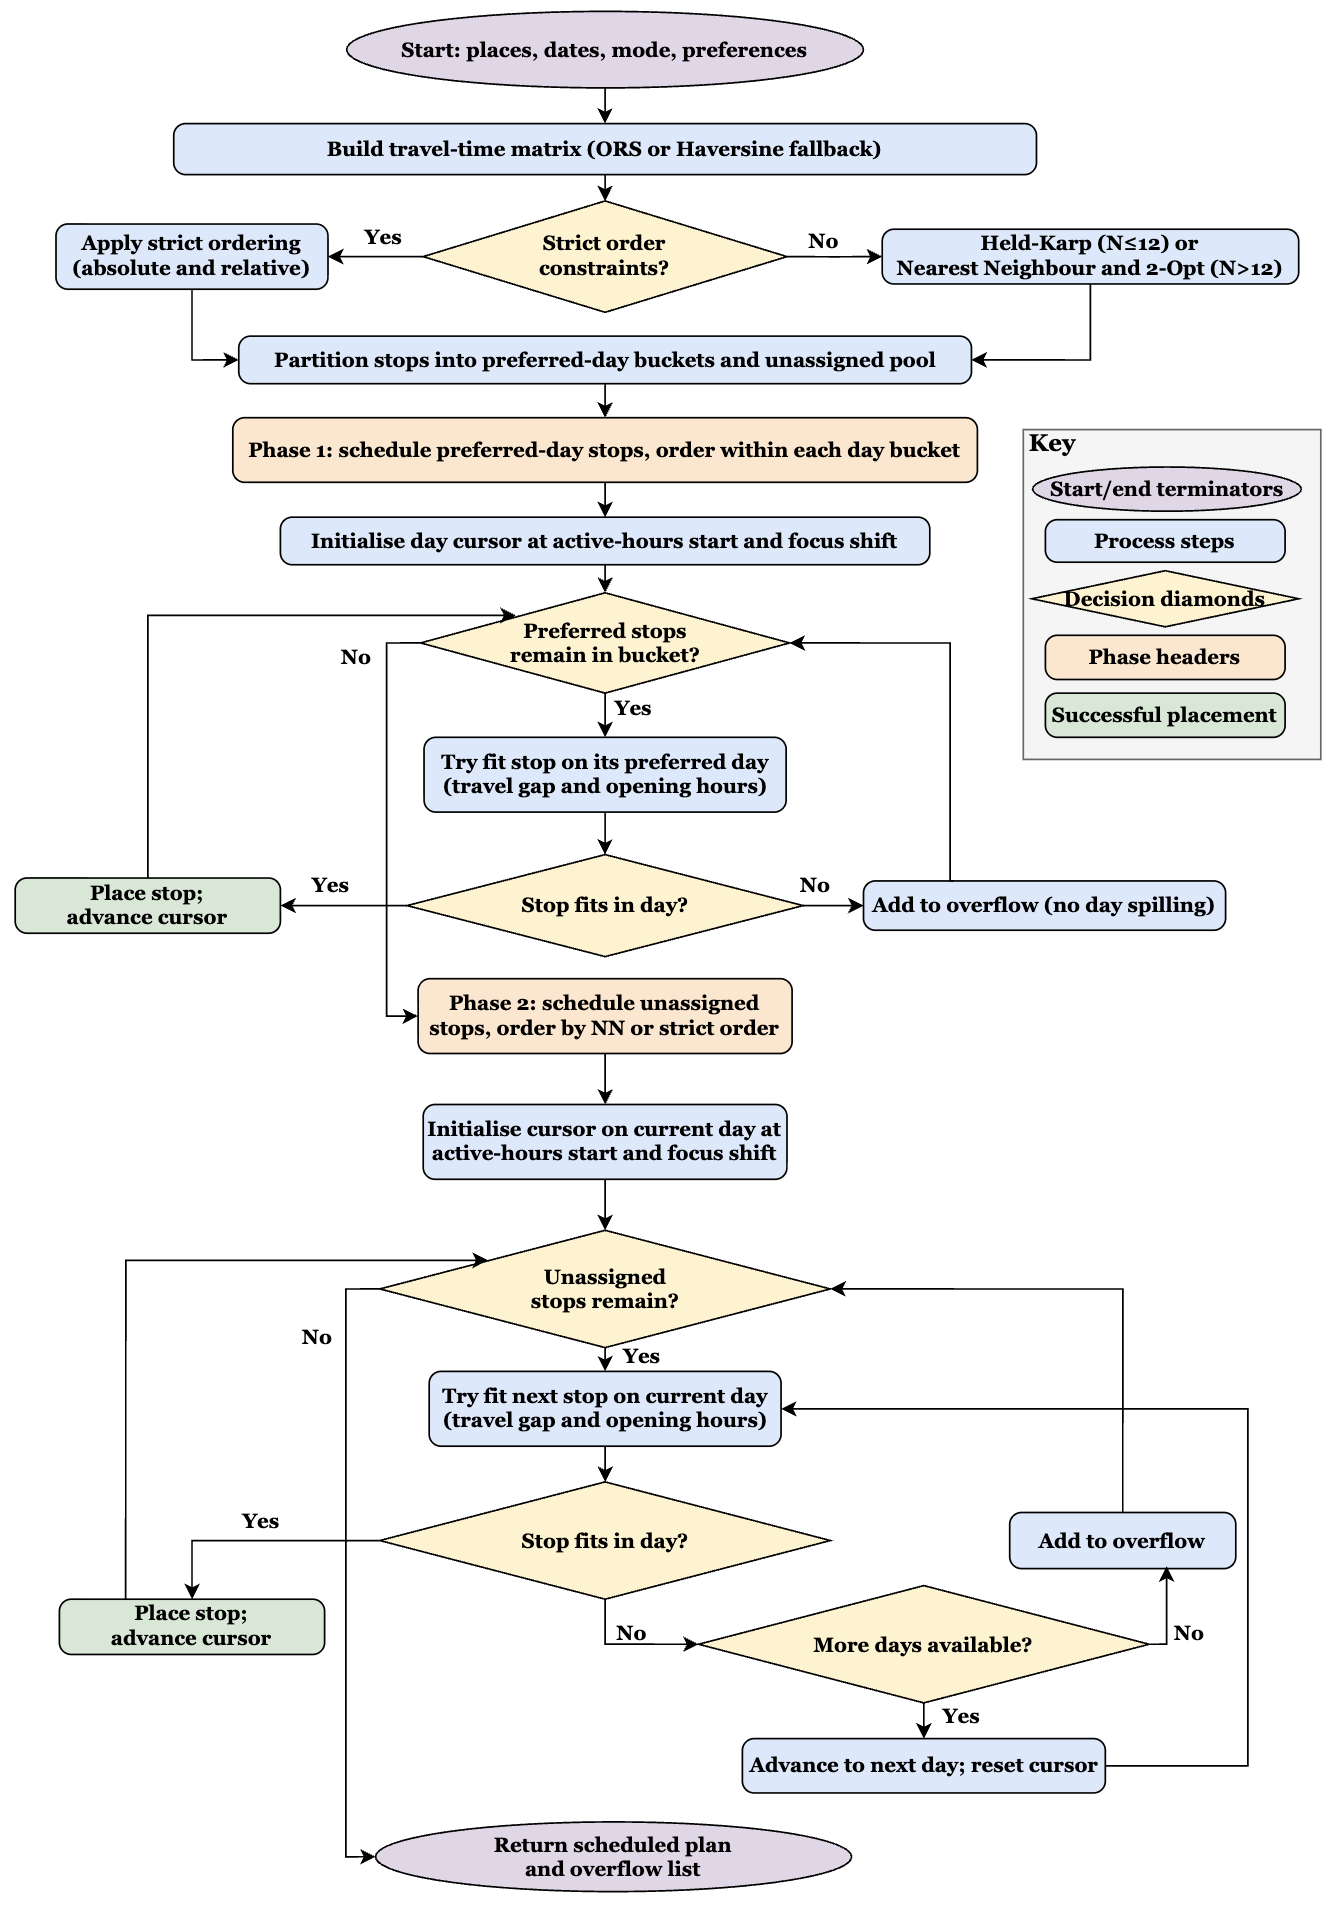
\includegraphics[width=0.9\textwidth]{Chapter6/auto-scheduler-flowchart.png}
  \caption{Auto-scheduler flowchart.}
  \label{fig:planner_flow}
\end{figure}

\begin{algorithm}[H]
  \caption{Auto-scheduler pseudocode (simplified from \texttt{server/planner.js}, 783~lines).}
  \label{alg:planner}
  \begin{algorithmic}[1]
    \Require $\mathit{places}$, $\mathit{days}$, $\mathit{activeStart}$, $\mathit{activeEnd}$, $\mathit{focus}$, $\mathit{transport}$
    \Ensure  $\mathit{days}$ (each with scheduled stops), $\mathit{overflow}$

    \Statex \Comment{--- Initialisation ---}
    \State $M \gets \Call{BuildTravelMatrix}{\mathit{places},\;\mathit{transport}}$
      \Comment{ORS or Haversine fallback}
    \If{$|\mathit{places}| \leq 12$}
      \State $\mathit{ordered} \gets \Call{HeldKarp}{\mathit{places},\;M}$
        \Comment{exact optimal order}
    \Else
      \State $\mathit{nnOrder} \gets \Call{NearestNeighbour}{\mathit{places},\;M}$
      \State $\mathit{ordered} \gets \Call{TwoOpt}{\mathit{nnOrder},\;M}$
    \EndIf
    \State partition $\mathit{ordered}$ into $\mathit{assignedByDay}$ and $\mathit{unassigned}$
    \State $\mathit{focusShift} \gets$ offset from $\mathit{focus}$
      \Comment{0, $\lfloor\mathit{span}/3\rfloor$, or $\lfloor\mathit{span}/1.8\rfloor$}

    \Statex
    \Statex \Comment{--- Phase 1: preferred-day stops ---}
    \For{each $\mathit{day}$ in $\mathit{days}$}
      \State $\mathit{cursor} \gets \mathit{activeStart} + \mathit{focusShift}$
      \For{each $\mathit{stop}$ in $\mathit{assignedByDay}[\mathit{day}]$}
        \State $\mathit{travel} \gets M[\mathit{last},\;\mathit{stop}]$
        \State $\mathit{propose} \gets \mathit{cursor} + \mathit{travel}$
        \State $(a, b, \mathit{fits}) \gets \Call{ApplyOpeningHours}{\mathit{stop},\;\mathit{propose},\;\mathit{activeEnd}}$
        \If{$\mathit{fits}$}
          \State schedule $\mathit{stop}$ at $[a, b]$; \; $\mathit{cursor} \gets b$
        \Else
          \State append $\mathit{stop}$ to $\mathit{overflow}$
        \EndIf
      \EndFor
    \EndFor

    \Statex
    \Statex \Comment{--- Phase 2: unassigned stops (greedy with spill) ---}
    \State $d \gets 0$; \; $\mathit{cursor} \gets \mathit{activeStart} + \mathit{focusShift}$
    \For{each $\mathit{stop}$ in $\mathit{unassigned}$}
      \State $\mathit{travel} \gets M[\mathit{last},\;\mathit{stop}]$
      \State $\mathit{propose} \gets \mathit{cursor} + \mathit{travel}$
      \State $(a, b, \mathit{fits}) \gets \Call{ApplyOpeningHours}{\mathit{stop},\;\mathit{propose},\;\mathit{activeEnd}}$
      \If{$\mathit{fits}$}
        \State schedule $\mathit{stop}$ on day $d$ at $[a, b]$; \; $\mathit{cursor} \gets b$
      \Else
        \While{$\lnot\mathit{fits}$ \textbf{and} $d < |\mathit{days}|$}
          \State $d \gets d + 1$; \; $\mathit{cursor} \gets \mathit{activeStart} + \mathit{focusShift}$
          \State $(a, b, \mathit{fits}) \gets \Call{ApplyOpeningHours}{\mathit{stop},\;\mathit{cursor},\;\mathit{activeEnd}}$
        \EndWhile
        \If{$\mathit{fits}$}
          \State schedule $\mathit{stop}$ on day $d$ at $[a, b]$; \; $\mathit{cursor} \gets b$
        \Else
          \State append $\mathit{stop}$ to $\mathit{overflow}$
        \EndIf
      \EndIf
    \EndFor

    \Statex
    \State \Return $(\mathit{days},\;\mathit{overflow})$
  \end{algorithmic}
\end{algorithm}

\section{Merge Implementation}
The merge engine is implemented in \texttt{server/merge.js}. Improvements made
after the Progress Report address known risks:
\begin{itemize}
  \item \textbf{Deep structural equality:} recursive comparison of nested
        objects, arrays, and primitives rather than reference equality
        (\texttt{===}) or \texttt{JSON.stringify}, which is sensitive to
        key ordering.
  \item \textbf{Robust stop identifiers:} if stops lack IDs, stable IDs are
        generated from name + coordinates + day context, reducing merge
        drop-outs.
  \item \textbf{Deterministic ordering:} days sorted by date; stops sorted by
        arrival time.
  \item \textbf{Deletion semantics:} explicit \texttt{plan-stop-delete} conflict
        for delete-vs-modify.
  \item \textbf{Field-level conflicts:} six selected fields (\texttt{name},
        \texttt{lat}, \texttt{lng}, \texttt{notes}, \texttt{stayMin},
        \texttt{routeMode}) produce \texttt{plan-stop-field} conflicts when both
        sides diverge.
\end{itemize}

Structural divergence is detected using a Jaccard similarity heuristic over
stop-key sets; if the Jaccard index falls below 0.4, a \texttt{plan-whole}
conflict is produced and the UI requires choosing an entire plan. Without this check, per-stop merging would attempt to align two largely unrelated itineraries, producing a nonsensical hybrid plan. For example, one collaborator completely replacing the plan with 5 new stops in Tokyo while the other completely replaces it with 5 new stops in Paris.

\begin{figure}[H]
  \centering
  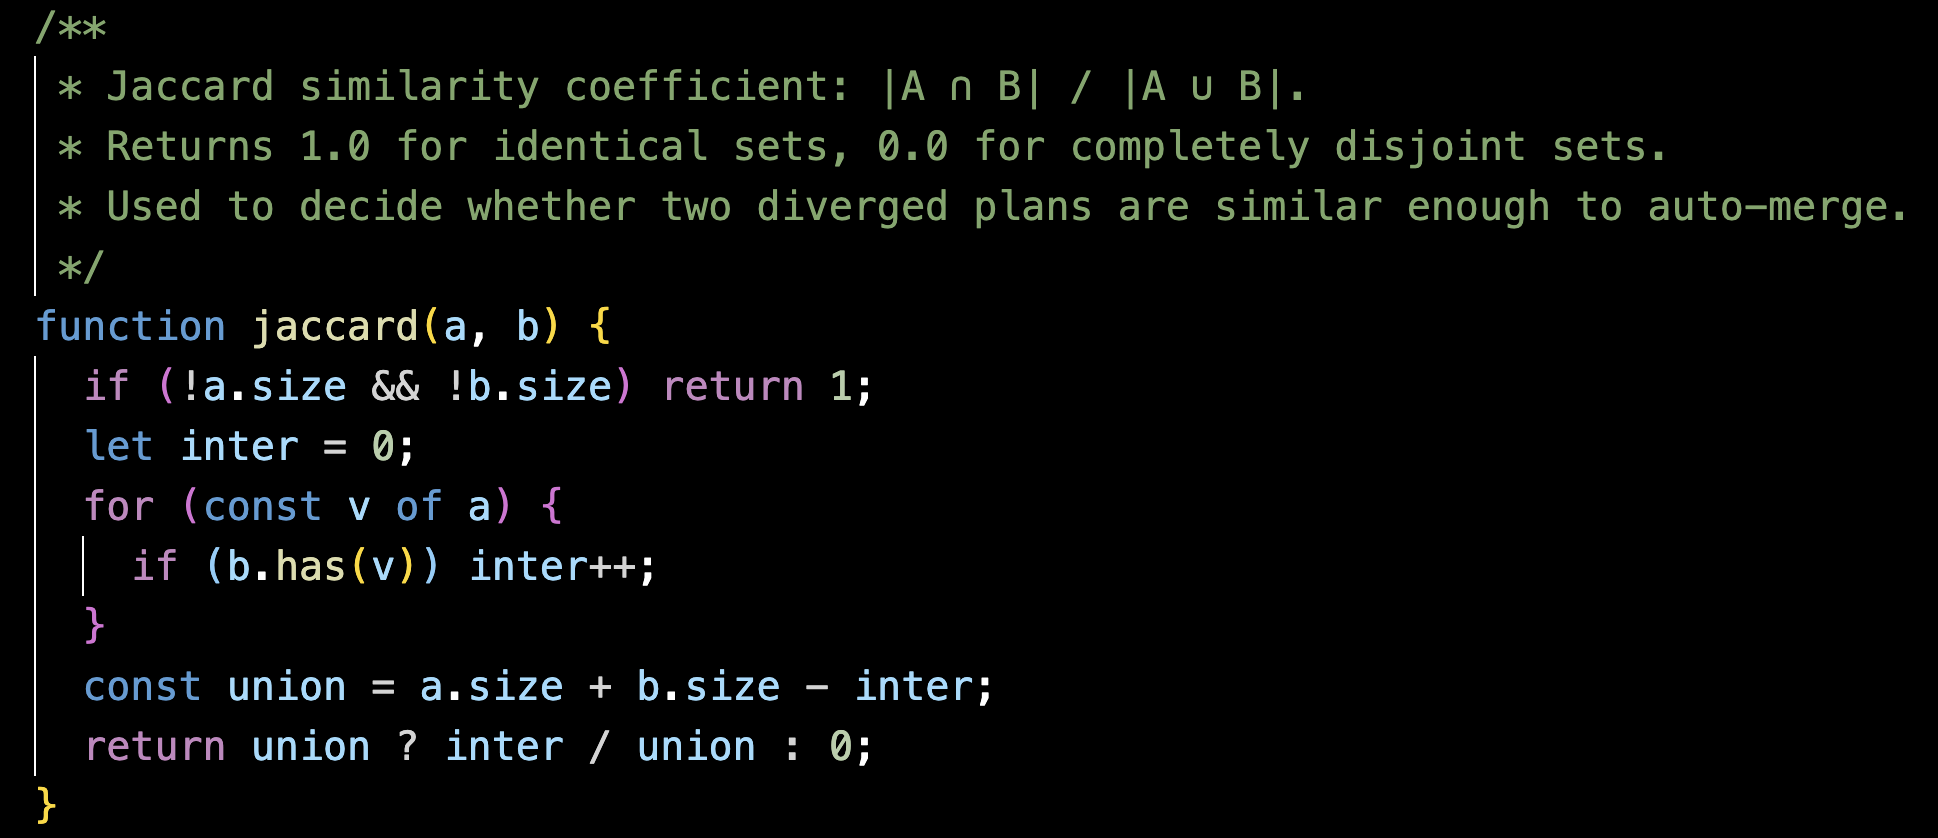
\includegraphics[width=0.85\linewidth]{Chapter6/jaccard-code.png}
  \caption{Jaccard similarity function (\texttt{server/merge.js}).}
  \label{fig:jaccard}
\end{figure}

\section{Routing Implementation}
Routing integration is implemented in \texttt{server/routing.js}:
\begin{itemize}
  \item ORS~\cite{ref_ors_matrix} matrix requests use the matrix endpoint and return durations in
        minutes.
  \item ORS directions requests fetch per-leg geometry for map rendering.
  \item Google Directions~\cite{ref_google_directions_api} transit routes provide detailed per-step segments,
        including polylines decoded via the standard polyline algorithm.
  \item Fallback estimates use Haversine distance with mode-dependent speed assumptions (approximately 5~km/h walking, 15~km/h cycling, 50~km/h driving, and 30~km/h transit).
\end{itemize}

\section{Quick Explore Mode}
Quick explore mode provides a Google-Maps-like workflow where users quickly enter
destinations, optimise an order, and optionally start a repository from the
result. This is implemented via \texttt{server/quickroute.js}:
\begin{itemize}
  \item for small instances (N $\leq$ 12), an exact Held-Karp dynamic programming
        solver is used \cite{ref_tsp_study,ref_tsp_local_search};
  \item for larger instances, NN is used with 2-Opt refinement
        \cite{ref_nn_2opt_hybrid}.
\end{itemize}

The quick route engine builds a travel-time matrix using ORS, transit pairwise
calls for small transit sets (limited to N~$\leq$~7 to control API cost), or
Haversine fallback. Concurrency is bounded to a pool of four simultaneous
requests to reduce API burst risk. The ordering logic reuses the same NN, 2-Opt, and Held-Karp strategies described in Section~\ref{sec:planner-impl} (Algorithms~\ref{alg:nn}--\ref{alg:heldkarp}).

\section{Algorithm Visualisation}
GiTrip includes an educational algorithm visualisation page
(\texttt{server/public/algorithm.js}) that demonstrates three route-ordering
algorithms with step-by-step animation on a Leaflet map:
\begin{enumerate}
  \item \textbf{Nearest Neighbour (NN):} greedy selection of the closest
        unvisited stop; $O(N^2)$ time.
  \item \textbf{NN and 2-Opt:} starts from an NN solution and iteratively reverses
        sub-segments to shorten the route; used for instances with more than 12
        stops.
  \item \textbf{Held-Karp dynamic programming (DP):} exact bitmask DP solver in
        $O(2^N \cdot N^2)$ time; guarantees optimality but is limited to
        N~$\leq$~12 stops due to exponential growth.
\end{enumerate}

The visualisation fetches real routing geometry from the server
(\texttt{/api/algo-matrix} and \texttt{/api/algo-geometry}), supports multiple
transport modes, and includes playback controls (play, pause, step, reset, speed
slider), synchronised pseudocode highlighting, animated scan lines showing which
edges are being evaluated, and a cost comparison panel.

\subsection{Constraint-Aware Scheduling Visualisation}
A second educational page (\texttt{/ui/schedule-demo}) demonstrates the
constraint-aware scheduling algorithm with eight animated scenarios:
\begin{enumerate}
  \item \textbf{Basic Schedule:} cursor-based packing with travel gaps.
  \item \textbf{Opening Hours:} nudging stops forward when proposed before
        opening time.
  \item \textbf{Fixed Time:} immovable stops that other stops pack around.
  \item \textbf{Time Windows:} soft desired-window preferences (e.g.\ lunch
        slot).
  \item \textbf{Day Overflow:} stops spilling to the next day when the active
        window is full.
  \item \textbf{Multi-Constraint:} opening hours, desired window, and fixed
        time combined in a single scenario.
  \item \textbf{Focus Shift:} comparing morning, midday, and afternoon start
        offsets side by side.
  \item \textbf{Compact vs Sparse:} comparing tight and distributed packing
        modes on the same stops.
\end{enumerate}

The page renders a Scalable Vector Graphics (SVG) day timeline (08:00--21:00 for demonstration) with animated stop blocks,
an opening-hours bar, a real-time constraint info panel, and synchronised
pseudocode highlighting. No API calls are required; all data is hardcoded.

\subsection{Three-Way Merge Visualisation}
A third educational page (\texttt{/ui/merge-demo}) demonstrates the three-way
merge algorithm with eight scenarios covering all merge outcomes:
\begin{itemize}
  \item \textbf{Auto-resolved:} clean merge (one side changed), identical
        changes (both made the same edit), and both-delete (both removed the
        same stop).
  \item \textbf{Conflicts:} stop-time conflict, delete-vs-edit conflict,
        field conflict (e.g.\ name differs), file conflict (e.g.\ trip
        description), and whole-plan conflict (Jaccard similarity below~0.4).
\end{itemize}

The page shows four plan panels (Base, Source, Target, Merged Result) with
colour-coded stop cards, animated per-stop comparison, and a file-level
description display for file-conflict scenarios. All three educational pages
share the same visual design, dark colour scheme, playback controls, and
pseudocode highlighting pattern, and are accessible via a ``How it works''
dropdown in the navigation bar.

\section{Frontend Implementation}
GiTrip's pages are server-rendered with EJS templates and enhanced with
client-side JavaScript:
\begin{itemize}
  \item \textbf{Repo UI:} displays trip plan, map, timeline, branches, commits,
        settings, and exports.
  \item \textbf{Merge UI:} presents conflicts and resolution controls, then
        submits a resolution payload to create a merge commit.
  \item \textbf{Planner UI:} collects inputs and submits to the planner endpoint
        to generate a new commit on a planner branch.
\end{itemize}

\subsection{Timeline and Map Editing}
The timeline editor uses draggable SVG elements with snapping to 5-minute
increments. It clamps edits based on travel constraints:
\begin{itemize}
  \item a stop cannot start before the previous stop's departure plus travel
        time,
  \item a stop cannot extend beyond the next stop's arrival,
  \item minimum stop duration is enforced.
\end{itemize}

The map editor uses Leaflet markers with numbered pins \cite{ref_leaflet}. In
edit mode, markers are draggable and route polylines are updated. Transit legs
display additional stop markers and per-leg mode styling (e.g., dashed walking
segments).

\section{Exports and PWA Features}
\subsection{PDF Export}
PDF export is implemented using browser printing (\texttt{window.print()}),
which is robust and avoids server-side rendering complexity.

\subsection{iCalendar Export}
GiTrip generates \texttt{text/calendar} content in iCalendar format and serves
it as an \texttt{.ics} download. The iCalendar format is defined by RFC 5545
\cite{ref_rfc5545}.

\subsection{PWA and Offline}
GiTrip includes PWA support through a web application manifest and a service
worker. The manifest standard is specified by W3C \cite{ref_appmanifest}, and
service workers are defined by W3C as an event-driven background worker model
enabling offline caching \cite{ref_service_workers}. Offline behaviour focuses
on caching core assets and recently accessed pages; limitations include the
inability to guarantee offline routing responses.

\section{Supporting Features}
\subsection{Weather Integration}
Each day in a plan displays a weather forecast retrieved from the Open-Meteo
API. The server fetches daily forecasts (temperature range, precipitation
probability, and weather code) using the first stop's coordinates for each day,
with a 30-minute Time-To-Live (TTL) cache to reduce external requests. Historical data is
fetched for past dates and forecast data for future dates.

\subsection{Travel Alerts}
GiTrip retrieves travel disruption news via the GNews API. City names are
extracted from stop names in the plan, and a search query combining those
cities with disruption keywords (strike, closure, protest, etc.) is issued.
Because articles about upcoming disruptions are typically published before
the affected dates, the search window extends from seven days before the
first trip date through the last trip date, and each article is assigned to the
nearest matching trip date. Results are displayed per day with badge counts.
Users can also add manual alert notes stored in the \texttt{travel\_alerts}
table.

\subsection{Public Gallery with Pagination}
The public gallery (\texttt{/ui/public}) displays trips that owners have
marked as public. The listing supports sorting by recency or star count and
is paginated at 12 trips per page using Structured Query Language (SQL) \texttt{LIMIT}/\texttt{OFFSET}
queries, preventing unbounded response sizes as the number of public trips
grows.

\section{Deployment and Operations}
GiTrip supports deployment via containerisation with a persistent volume for the
SQLite database file (\texttt{gitrip.db}). The server starts on \texttt{PORT}
(default 4000) and automatically increments if the port is in use. Environment
variables provide routing API keys. The system was deployed for Evaluation Day to
allow participants to access the application from multiple machines and personal
devices.

% !TEX root = ../Report.tex
% ======================================================================
\chapter{Testing}
% ======================================================================

This chapter provides evidence that GiTrip was tested systematically at unit,
functional, and non-functional levels. The goal is to demonstrate correctness for
core algorithms (merge and scheduler) and reliability for user-facing workflows.

\section{Unit Testing}
GiTrip includes five unit test files with 64 test cases total, executed using
the Node.js native test framework (\texttt{node:test}) with strict assertions.

\begin{table}[H]
\centering
\caption{Summary of unit test coverage (64 test cases).}
\label{tab:unit_tests_summary}
\begin{tabular}{@{}p{0.30\linewidth}p{0.50\linewidth}p{0.12\linewidth}@{}}
\toprule
\textbf{Test file} & \textbf{Primary coverage} & \textbf{\# tests} \\
\midrule
\texttt{openhours.test.js} & Opening-hours parsing and interval validation & 11 \\
\texttt{merge.test.js}     & Three-way merge and conflict detection        & 16 \\
\texttt{planner.test.js}   & Time utilities and opening-hours scheduling   & 13 \\
\texttt{routing.test.js}   & Haversine fallback and constant-gap defaults  & 11 \\
\texttt{api-keys.test.js}  & External API connectivity (ORS, Google, GNews, Open-Meteo, Nominatim) & 13 \\
\midrule
\textbf{Total} &  & \textbf{64} \\
\bottomrule
\end{tabular}
\end{table}

\subsection{Opening Hours Parsing and Validation}
The opening-hours module tests include:
\begin{itemize}
  \item standard weekday ranges (e.g., \texttt{Mo-Fr 09:00-18:00}),
  \item wrap-around ranges (e.g., \texttt{Fr-Mo}),
  \item \texttt{off} keyword meaning closed,
  \item multi-span days with breaks,
  \item compound rules across different days,
  \item empty/null input handling.
\end{itemize}

Validation tests check whether a proposed interval is open, closed, nudged to a
next open slot, too long to fit, or exactly fits a boundary.

\subsection{Merge Conflict Detection}
Merge tests cover:
\begin{itemize}
  \item clean merges where only one side changes,
  \item deep-equality behaviour that is independent of key order,
  \item deletions (delete-vs-modify yields explicit
        \texttt{plan-stop-delete} conflict),
  \item time conflicts (\texttt{plan-stop-time}),
  \item field conflicts (\texttt{plan-stop-field}),
  \item whole-plan conflicts when similarity is low (\texttt{plan-whole}),
  \item deterministic ordering of merged days and stops.
\end{itemize}

\subsection{Planner Time Utilities and Scheduling Logic}
Planner tests cover both time-conversion functions (\texttt{toMin},
\texttt{toHHMM}, including null/empty inputs, negative clamping, and fractional
rounding) and the \texttt{applyOpeningHours} constraint engine, including:
\begin{itemize}
  \item unconstrained scheduling (no constraints; starts at proposed arrival),
  \item clamping to active period,
  \item soft desired windows (\texttt{desiredStart}, \texttt{desiredEnd}),
  \item opening-hours nudging to the next open slot,
  \item hard fixed-time windows (failure when travel arrives too late),
  \item rejection when the stop does not fit within the active window,
  \item rejection when the venue is closed all day.
\end{itemize}

\subsection{Routing Fallback Logic}
Routing tests cover the Haversine fallback estimator and constant-gap defaults
used when external routing APIs are unavailable:
\begin{itemize}
  \item identity case (same point returns zero travel time),
  \item realistic distance estimation (London to Paris within expected range),
  \item mode ordering (walking slower than cycling, cycling slower than driving),
  \item graceful handling of null or missing coordinates,
  \item constant-gap values for each transport mode.
\end{itemize}

\subsection{External API Connectivity}
API connectivity tests verify that every third-party service required by GiTrip
is correctly configured and reachable at test time:
\begin{itemize}
  \item \textbf{Presence checks} -- each required environment variable
        (\texttt{ORS\_API\_KEY}, \texttt{GOOGLE\_DIRECTIONS\_API\_KEY},
        \texttt{NEWS\_API\_KEY}) is set in \texttt{.env}.
  \item \textbf{ORS (OpenRouteService)} -- a real matrix request and a
        directions request confirm the key is accepted and returns valid
        duration data.
  \item \textbf{Google Directions} -- both driving and transit modes are
        tested; the test asserts that the response status is \texttt{OK}
        (not \texttt{REQUEST\_DENIED}), catching billing or API-enablement
        issues early.
  \item \textbf{GNews} -- a search query confirms the key returns articles
        and a travel-specific query returns relevant results.
  \item \textbf{Open-Meteo} -- both the forecast and archive endpoints are
        tested with a London coordinate, verifying that daily temperature
        and precipitation data are returned in the expected format.
  \item \textbf{Nominatim} -- a geocoding search confirms the endpoint
        returns results with latitude, longitude, and display name. A
        second test verifies that the \texttt{extratags} field (which
        carries opening-hours data from OSM) is present when requested.
\end{itemize}
These tests act as a deployment smoke test: a single failing assertion
pinpoints exactly which external service is misconfigured, rather than
requiring manual investigation of silent routing fallbacks.

\section{Functional Testing}
Functional testing verified that core workflows operate end-to-end.
Table~\ref{tab:functional_tests} summarises key cases.

\begin{table}[H]
\centering
\caption{Functional test cases for core workflows (summary).}
\label{tab:functional_tests}
\begin{tabular}{@{}p{0.52\linewidth}p{0.18\linewidth}p{0.22\linewidth}@{}}
\toprule
\textbf{Workflow} & \textbf{Result} & \textbf{Evidence} \\
\midrule
Create repo; view/edit tabs render              & Pass & Manual verification \\
Run auto-planner; commit created; redirect      & Pass & Commit history updated \\
Timeline edit; save commit; reload matches      & Pass & Snapshot persists \\
Map marker drag; recompute route; save          & Pass & Geometry updates \\
Create branch; switch branch; plan changes      & Pass & Head snapshot changes \\
Merge branches with time conflict; resolve      & Pass & Conflict UI + merge commit \\
Quick explore optimise; start repo from route   & Pass & Repo created from route \\
Export PDF view                                 & Pass & Browser print output \\
Export iCalendar (ICS)                          & Pass & Calendar import works \\
\bottomrule
\end{tabular}
\end{table}

\section{Non-functional Testing and Checks}
\subsection{Security Checks}
GiTrip includes:
\begin{itemize}
  \item Content Security Policy headers and anti-framing headers,
  \item four-tier rate limiting (global, API, geo search, and authentication
        endpoints),
  \item prepared statements for all database access,
  \item conservative input normalisation for user-provided fields,
  \item generic error messages in all user-facing responses (internal details
        logged server-side only, preventing information leakage).
\end{itemize}

These checks are not a substitute for a full penetration test, but they provide
reasonable baseline hardening for a deployed student project.

\subsection{Accessibility Checks}
Accessibility was guided by WCAG 2.2 \cite{ref_wcag22}. Checks included:
\begin{itemize}
  \item consistent labelling of controls,
  \item avoiding information conveyed only via colour,
  \item readable typography and spacing,
  \item basic keyboard navigation for non-map interactions.
\end{itemize}

A more formal audit using automated tools such as Lighthouse is recommended for
future work \cite{ref_lighthouse_overview}. The interactive map and timeline
remain difficult to fully validate for accessibility within the project scope.

\subsection{Resilience to External API Failures}
Functional tests included scenarios where routing keys were missing or external
calls failed. In these cases, GiTrip falls back to approximate travel-time
estimates and still produces a schedule (potentially with reduced accuracy). This
behaviour supports usability in constrained environments.

\section{Testing Summary}
The testing evidence demonstrates that the most error-prone components (merge
logic and scheduler constraints) are covered by automated unit tests and that
major user workflows function end-to-end. Remaining limitations are largely
usability and accessibility challenges inherent in interactive planning UIs,
rather than basic correctness failures.

% !TEX root = ../Report.tex
% ======================================================================
\chapter{Evaluation}
% ======================================================================

This chapter reports the evaluation conducted on Evaluation Day (Wednesday 25th
February 2026) and via a follow-up survey. It presents both objective user
acceptance test results and subjective survey findings, and interprets them
against the project's success criteria.

\section{Evaluation Day Setup}
Evaluation Day took place in the Department of Computer Science, Room CS0.03,
Table B01, slot 13:05--13:45, with the project titled ``GiTrip --- Git for
Collaborative Trip Planning''. The demonstration environment used four Linux
machines plus the author's laptop so that multiple participants could test
branching and merging behaviours in parallel. Additionally, the application was
deployed publicly so attendees could also use their own laptops and devices.

\section{Participants}
Two data sources were collected:
\begin{itemize}
  \item \textbf{User Acceptance Test (UAT):} 10 in-person participants (P1--P10)
        with observer-recorded results.
  \item \textbf{Survey responses:} 13 responses collected via Microsoft Forms
        (including remote responses). The survey reported an average completion
        time of 08:46 minutes.
\end{itemize}

Survey respondents had mixed Git familiarity: 2 not familiar, 5 somewhat
familiar, 3 comfortable, and 3 very comfortable.

\section{User Acceptance Testing Tasks}
Three tasks were measured using an observer checklist to provide objective
evidence.

\subsection{Task T1: Auto-schedule Feasibility}
Scenario: at least six stops across one to two days. Evidence recorded:
completion, time-to-finish, non-overlap, and non-zero travel gaps.

\begin{table}[H]
\centering
\caption{UAT Task T1 --- Auto-schedule feasibility.}
\label{tab:uat_t1}
\begin{tabular}{@{}lcccc@{}}
\toprule
\textbf{Participant} & \textbf{Completed?} & \textbf{Time} &
\textbf{Non-overlapping?} & \textbf{Non-zero travel gaps?} \\
\midrule
P1  & Y & 3:12  & Y & Y \\
P2  & Y & 4:45  & Y & Y \\
P3  & Y & 2:58  & Y & Y \\
P4  & Y & 5:30  & Y & Y \\
P5  & Y & 3:44  & Y & Y \\
P6  & Y & 6:02  & Y & Y \\
P7  & N & 8:00* & -- & -- \\
P8  & Y & 4:11  & Y & Y \\
P9  & Y & 3:55  & Y & Y \\
P10 & Y & 4:28  & Y & Y \\
\bottomrule
\end{tabular}

\vspace{0.3em}
{\footnotesize *P7 timed out due to difficulty locating the auto-scheduler
button without a hint.}
\end{table}

Across successful completions (9/10), the mean completion time was 4:18 (median
4:11), and all successful outputs were non-overlapping with non-zero travel gaps.
This supports Success Criterion SC2.

\subsection{Task T2: Merge Conflict Resolution}
Scenario: pre-seeded repository with two branches producing at least one timing
conflict. Evidence recorded: resolved or not, time-to-resolve, and number of
hints given.

\begin{table}[H]
\centering
\caption{UAT Task T2 --- Merge conflict resolution.}
\label{tab:uat_t2}
\begin{tabular}{@{}lccc@{}}
\toprule
\textbf{Participant} & \textbf{Resolved?} & \textbf{Time} &
\textbf{Hints given} \\
\midrule
P1  & Y & 2:34  & 0 \\
P2  & Y & 4:50  & 1 \\
P3  & Y & 1:58  & 0 \\
P4  & Y & 3:22  & 0 \\
P5  & Y & 4:47  & 1 \\
P6  & N & 6:10* & 2 \\
P7  & Y & 3:05  & 1 \\
P8  & Y & 2:41  & 0 \\
P9  & Y & 4:33  & 1 \\
P10 & Y & 3:18  & 0 \\
\bottomrule
\end{tabular}

\vspace{0.3em}
{\footnotesize *P6 selected the wrong branch and ran out of time.}
\end{table}

Overall, 9/10 participants resolved the conflict; 9/10 achieved a resolution
within 5 minutes. The mean time across all participants was 3:44 (mean hints
0.6). This supports Success Criterion SC1.

\subsection{Task T3: Quick Edit + Save Without Git Explanation}
Task T3 measured whether a participant could make a small timeline/map edit and
save without requiring Git vocabulary explanation.

\begin{table}[H]
\centering
\caption{UAT Task T3 --- Quick edit and save without Git explanation.}
\label{tab:uat_t3}
\begin{tabular}{@{}lcp{0.60\linewidth}@{}}
\toprule
\textbf{Participant} & \textbf{Completed?} & \textbf{Notes} \\
\midrule
P1  & Y & Edited timeline stop duration naturally \\
P2  & Y & Used ``Save'' without prompting \\
P3  & Y & -- \\
P4  & N & Asked ``does saving here create a version?'' \\
P5  & Y & -- \\
P6  & Y & -- \\
P7  & Y & -- \\
P8  & N & Hesitated; unsure if edit was auto-saved \\
P9  & Y & -- \\
P10 & Y & -- \\
\bottomrule
\end{tabular}
\end{table}

8/10 completed without needing Git explanation. This supports the value of Easy
mode and indicates that versioning concepts can still raise questions (notably
around mental models of saving).

\section{Survey Results}
The Evaluation Day survey collected 13 responses. Key quantitative findings
included:
\begin{itemize}
  \item Git familiarity was mixed: 15\% not familiar (2/13), 38\% somewhat
        familiar (5/13), 23\% comfortable (3/13), 23\% very comfortable (3/13).
  \item Participants tried a range of features: 11 created/opened a repository,
        9 ran the auto-scheduler, 5 attempted branch/compare and merge/conflict
        resolution, and 4 used quick route mode.
\end{itemize}

Likert responses across Core Functionality and Overall Impression were strongly
positive, with responses concentrated in Agree/Strongly Agree. The Git Concept
Understanding section was also positive but showed more neutral responses,
suggesting that the conceptual model is understandable but still benefits from
guidance for some users.

The survey included the System Usability Scale (SUS). Due to the small sample
size and the visual aggregation format, this report interprets SUS qualitatively
rather than claiming a statistically robust SUS score. The overall pattern
indicates that positive usability statements were generally endorsed while
negative statements about complexity and inconsistency were generally rejected.

\subsection{Qualitative Feedback}
Free-text responses provide additional evidence of perceived value and pain
points. Representative themes include:

\textbf{Most useful/impressive:}
\begin{itemize}
  \item Auto-scheduler usefulness and edge-case handling (e.g., clearly showing
        unscheduled stops with reasons).
  \item Novelty of Git-style planning and merge conflict resolution in a non-code
        context.
  \item Educational value of algorithm visualisation.
\end{itemize}

\textbf{Most frustrating:}
\begin{itemize}
  \item Some users perceived Git concepts as requiring learning overhead.
  \item Merge conflicts can be confusing without guidance (consistent with UAT
        hint patterns).
  \item A routing limitation was reported for special transport modes (e.g.,
        ferries), reflecting dependency on external routing providers.
\end{itemize}

\textbf{Would users adopt GiTrip?} Most respondents indicated ``yes'' or
``maybe'', with collaboration and ``keeping everything in one place'' cited as
major benefits. The strongest blockers were perceived complexity for casual trips
and routing-provider constraints for niche transport types.

\section{Discussion Against Success Criteria}
Overall, the evaluation provides strong evidence that core objectives were
achieved:
\begin{itemize}
  \item The auto-scheduler reliably produced feasible plans for typical scenarios
        (SC2 met).
  \item Merge conflict resolution was achievable by most participants within the
        target time (SC1 met).
  \item Usability feedback validates the Easy mode approach while highlighting
        discoverability and conceptual learning as remaining improvement areas
        (SC3 partially met, with known limitations).
\end{itemize}

\section{Threats to Validity}
The evaluation has limitations typical of student project evaluations:
\begin{itemize}
  \item \textbf{Sample bias:} many participants were likely students with
        above-average technical literacy.
  \item \textbf{Small sample size:} limits statistical confidence, especially
        for SUS scoring.
  \item \textbf{Demonstration context:} users may perform differently in real
        trip planning over longer time horizons.
\end{itemize}

Despite these limitations, the objective task results and consistent qualitative
themes together support the conclusion that the core objectives were met.

% !TEX root = ../Report.tex
% ======================================================================
\chapter{Conclusions and Future Work}
% ======================================================================

This chapter summarises achievements, critiques the system against its goals,
discusses limitations, and proposes future work.

\section{Conclusions}
GiTrip demonstrates that Git-like version control semantics can be meaningfully
applied to collaborative trip planning. The completed system meets the Must-have
objectives from the Project Specification:
\begin{itemize}
  \item repository-based trip storage with commits and branches,
  \item constraint-aware automatic scheduling integrating routing data,
  \item interactive timeline and map editing with commit saving,
  \item three-way merge with a dedicated conflict-resolution UI.
\end{itemize}

Evaluation results provide objective evidence that users can successfully
generate feasible itineraries and resolve merge conflicts within target times.
Survey feedback confirms perceived novelty and practical value, particularly for
group trips and scenarios requiring careful coordination.

\section{Critical Reflection and Lessons Learned}
Several lessons emerged during development and evaluation:
\begin{itemize}
  \item \textbf{Git concepts are powerful but cognitively expensive.} During
        Evaluation Day, even participants who understood the UI hesitated when
        encountering terms like branch and merge. The Easy mode toggle proved
        essential, but discoverability and mental model support remain ongoing
        work.
  \item \textbf{Structured merge is domain-specific.} Early iterations used
        \texttt{JSON.stringify}-based comparison, which caused subtle bugs when
        key ordering differed between branches. Switching to deep structural
        equality, stable IDs, and explicit deletion semantics resolved these
        issues but required substantial reworking of the merge engine.
  \item \textbf{Constraint scheduling requires explainability.} Feedback from
        testing showed that users trusted the auto-scheduler more when
        adjustments (e.g., opening-hours nudges) were visibly annotated with
        reasons.
  \item \textbf{External dependency management matters.} During development,
        OpenRouteService rate limits and occasional Google Directions failures
        highlighted the need for Haversine-based fallback strategies to keep the
        planner usable under degraded conditions.
\end{itemize}

\section{Limitations}
Key limitations include:
\begin{itemize}
  \item \textbf{Accessibility of interactive components:} maps and drag-based
        timelines remain challenging for keyboard-only and screen-reader users.
  \item \textbf{Merge granularity trade-offs:} while field-level conflicts are
        supported for selected fields, a fully general per-field resolver could
        overwhelm users.
  \item \textbf{No real-time collaboration:} GiTrip supports asynchronous
        collaboration via branches and merges, but not simultaneous live editing
        (CRDT/OT).
  \item \textbf{Heuristic scheduling:} the planner prioritises feasibility and
        responsiveness over global optimality.
\end{itemize}

\section{Future Work}
Future work opportunities are substantial:
\begin{itemize}
  \item \textbf{Improved onboarding and guidance:} in-product tutorials for
        branching/merging, contextual tips, and clearer ``Save'' semantics to
        reduce confusion.
  \item \textbf{Accessibility enhancements:} keyboard-operable alternatives for
        timeline edits, text-based route editing, and stronger ARIA support.
  \item \textbf{Real-time collaboration:} explore CRDT-based shared plan editing,
        while preserving a mergeable history model.
  \item \textbf{Richer merge resolution:} expand conflict detection to additional
        fields, include conflict previews, and support partial merges.
  \item \textbf{Routing extensions:} support ferries/planes as explicit legs,
        integrate GTFS-based transit where applicable, and improve offline routing
        approximations.
  \item \textbf{Optional ML/AI extensions:} while excluded from the MVP, future
        versions could use machine learning to:
        \begin{itemize}
          \item learn user preferences (pace, activity types) and suggest better
                defaults,
          \item predict realistic dwell times and travel-time uncertainty,
          \item recommend destinations based on context (with careful privacy
                design).
        \end{itemize}
        These ideas should be implemented cautiously to maintain explainability
        and avoid undermining deterministic feasibility guarantees.
\end{itemize}

% ======================================================================
\chapter*{Author's Assessment of the Project}
\addcontentsline{toc}{chapter}{Author's Assessment of the Project}
% ======================================================================

\textbf{What is the (technical) contribution of this project?} GiTrip contributes
a practical system that applies Git-style branching, committing, and three-way
merging to structured itinerary data, integrated with constraint-aware scheduling
and interactive timeline/map editing.

\textbf{Why is this contribution relevant to Computer Science?} The project
connects software configuration management concepts (history, merging, conflict
resolution) with human-centred planning, demonstrating how domain semantics
change the design of storage, algorithms, and user interfaces.

\textbf{How can others make use of the work?} Developers can reuse the
snapshot-based repository model, merge engine patterns for structured JSON, and
the planner's constraint-handling approach in other collaborative planning
domains.

\textbf{Why should this project be considered an achievement?} It delivers an
end-to-end deployed application combining routing integration, a scheduler, and a
merge UI; evaluation shows users can complete core tasks successfully with limited
guidance.

\textbf{What are the limitations?} The main limitations are accessibility for
interactive controls, dependence on external routing providers, and the absence
of real-time collaboration and AI-based recommendation within the MVP scope.


% Back Matter (excluded from word count)
\bibliographystyle{ieeetr}
\bibliography{bibliography}

% !TEX root = ../Report.tex
\appendix

\chapter{Evaluation Day Survey Instrument and Results}
\label{appx:survey}

This appendix contains supporting evidence from the Evaluation Day survey. The
main body of the report presents the key findings; the complete survey export is
included here to allow assessors to inspect the full distribution of responses.

\section{Survey Questions (Summary)}
The survey included:
\begin{itemize}
  \item Git familiarity and feature usage questions,
  \item System Usability Scale (SUS) items,
  \item Git concept understanding Likert items,
  \item Core functionality Likert items,
  \item Overall impression Likert items,
  \item free-text questions on positives, frustrations, adoption likelihood,
        and comparison to current workflows.
\end{itemize}

\section{Full Survey Export PDF}
\textbf{Compilation note:} place \texttt{eval\_day\_survey\_results.pdf} in the
same directory as this \texttt{.tex} file, or update the path below.

% Uncomment the line below once the PDF is available:
% \includepdf[pages=-]{Appendices/eval_day_survey_results.pdf}

\chapter{User Acceptance Test Results (Full Tables)}
\label{appx:uat}

This appendix reproduces the full UAT results from Evaluation Day for archival
completeness. Summary statistics are presented in Chapter~8; the raw data is
included here to allow detailed inspection.

\begin{table}[H]
\centering
\caption{UAT Task T1 --- Auto-schedule feasibility (full results).}
\begin{tabular}{@{}lcccc@{}}
\toprule
\textbf{Participant} & \textbf{Completed?} & \textbf{Time} &
\textbf{Non-overlapping?} & \textbf{Non-zero travel gaps?} \\
\midrule
P1  & Y & 3:12  & Y & Y \\
P2  & Y & 4:45  & Y & Y \\
P3  & Y & 2:58  & Y & Y \\
P4  & Y & 5:30  & Y & Y \\
P5  & Y & 3:44  & Y & Y \\
P6  & Y & 6:02  & Y & Y \\
P7  & N & 8:00* & -- & -- \\
P8  & Y & 4:11  & Y & Y \\
P9  & Y & 3:55  & Y & Y \\
P10 & Y & 4:28  & Y & Y \\
\bottomrule
\end{tabular}

\vspace{0.3em}
{\footnotesize *P7 timed out due to difficulty locating the auto-scheduler
button without a hint.}
\end{table}

\begin{table}[H]
\centering
\caption{UAT Task T2 --- Merge conflict resolution (full results).}
\begin{tabular}{@{}lccc@{}}
\toprule
\textbf{Participant} & \textbf{Resolved?} & \textbf{Time} &
\textbf{Hints given} \\
\midrule
P1  & Y & 2:34  & 0 \\
P2  & Y & 4:50  & 1 \\
P3  & Y & 1:58  & 0 \\
P4  & Y & 3:22  & 0 \\
P5  & Y & 4:47  & 1 \\
P6  & N & 6:10* & 2 \\
P7  & Y & 3:05  & 1 \\
P8  & Y & 2:41  & 0 \\
P9  & Y & 4:33  & 1 \\
P10 & Y & 3:18  & 0 \\
\bottomrule
\end{tabular}

\vspace{0.3em}
{\footnotesize *P6 selected the wrong branch and ran out of time.}
\end{table}

\begin{table}[H]
\centering
\caption{UAT Task T3 --- Quick edit and save without Git explanation (full
results).}
\begin{tabular}{@{}lcp{0.55\linewidth}@{}}
\toprule
\textbf{Participant} & \textbf{Completed?} & \textbf{Notes} \\
\midrule
P1  & Y & Edited timeline stop duration naturally \\
P2  & Y & Used ``Save'' without prompting \\
P3  & Y & -- \\
P4  & N & Asked ``does saving here create a version?'' \\
P5  & Y & -- \\
P6  & Y & -- \\
P7  & Y & -- \\
P8  & N & Hesitated; unsure if edit was auto-saved \\
P9  & Y & -- \\
P10 & Y & -- \\
\bottomrule
\end{tabular}
\end{table}

\chapter{Additional Diagrams and Screenshots}
\label{appx:diagrams}

% TODO: Replace each placeholder below with a real screenshot.
%       Save screenshots as PNG/PDF in the Appendices/ folder and use:
%       \includegraphics[width=0.92\linewidth]{Appendices/filename.png}

\begin{figure}[H]
  \centering
  % 
\includegraphics[width=0.92\linewidth]{Appendices/merge-ui.png}
  \fbox{\parbox{0.92\linewidth}{\centering TODO: screenshot of the merge
  conflict resolution UI showing ours/theirs choices and the resolve button.}}
  \caption{Merge conflict resolution UI.}
\end{figure}

\begin{figure}[H]
  \centering
  % \includegraphics[width=0.92\linewidth]{Appendices/timeline-editor.png}
  \fbox{\parbox{0.92\linewidth}{\centering TODO: screenshot of the timeline
  editor with draggable stop blocks showing arrival/departure times.}}
  \caption{Timeline editor with draggable stop blocks.}
\end{figure}

\begin{figure}[H]
  \centering
  % \includegraphics[width=0.92\linewidth]{Appendices/map-editor.png}
  \fbox{\parbox{0.92\linewidth}{\centering TODO: screenshot of the map editor
  showing numbered markers, route polylines, and transit leg styling.}}
  \caption{Map editor with numbered markers and route geometry.}
\end{figure}

\begin{figure}[H]
  \centering
  % \includegraphics[width=0.92\linewidth]{Appendices/easy-mode.png}
  \fbox{\parbox{0.92\linewidth}{\centering TODO: screenshot comparing Easy mode
  (simplified controls) vs Git mode (branches, commits, merge visible).}}
  \caption{Easy mode vs Git mode comparison.}
\end{figure}

\begin{figure}[H]
  \centering
  % \includegraphics[width=0.92\linewidth]{Appendices/algo-visualisation.png}
  \fbox{\parbox{0.92\linewidth}{\centering TODO: screenshot of the algorithm
  visualisation page showing the map, pseudocode highlighting, and playback
  controls.}}
  \caption{Algorithm visualisation page.}
\end{figure}

\begin{figure}[H]
  \centering
  % \includegraphics[width=0.92\linewidth]{Appendices/quick-explore.png}
  \fbox{\parbox{0.92\linewidth}{\centering TODO: screenshot of the quick
  explore mode showing the optimised route with summary stats.}}
  \caption{Quick explore mode with optimised route.}
\end{figure}

\chapter{Project Schedule}
\label{appx:schedule}

Figure~\ref{fig:gantt} shows the project timeline across the two terms of the
2025/26 academic year. Table~\ref{tab:schedule_detail} provides a breakdown of
deliverables per phase.

\begin{figure}[H]
  \centering
  \resizebox{\textwidth}{!}{%
  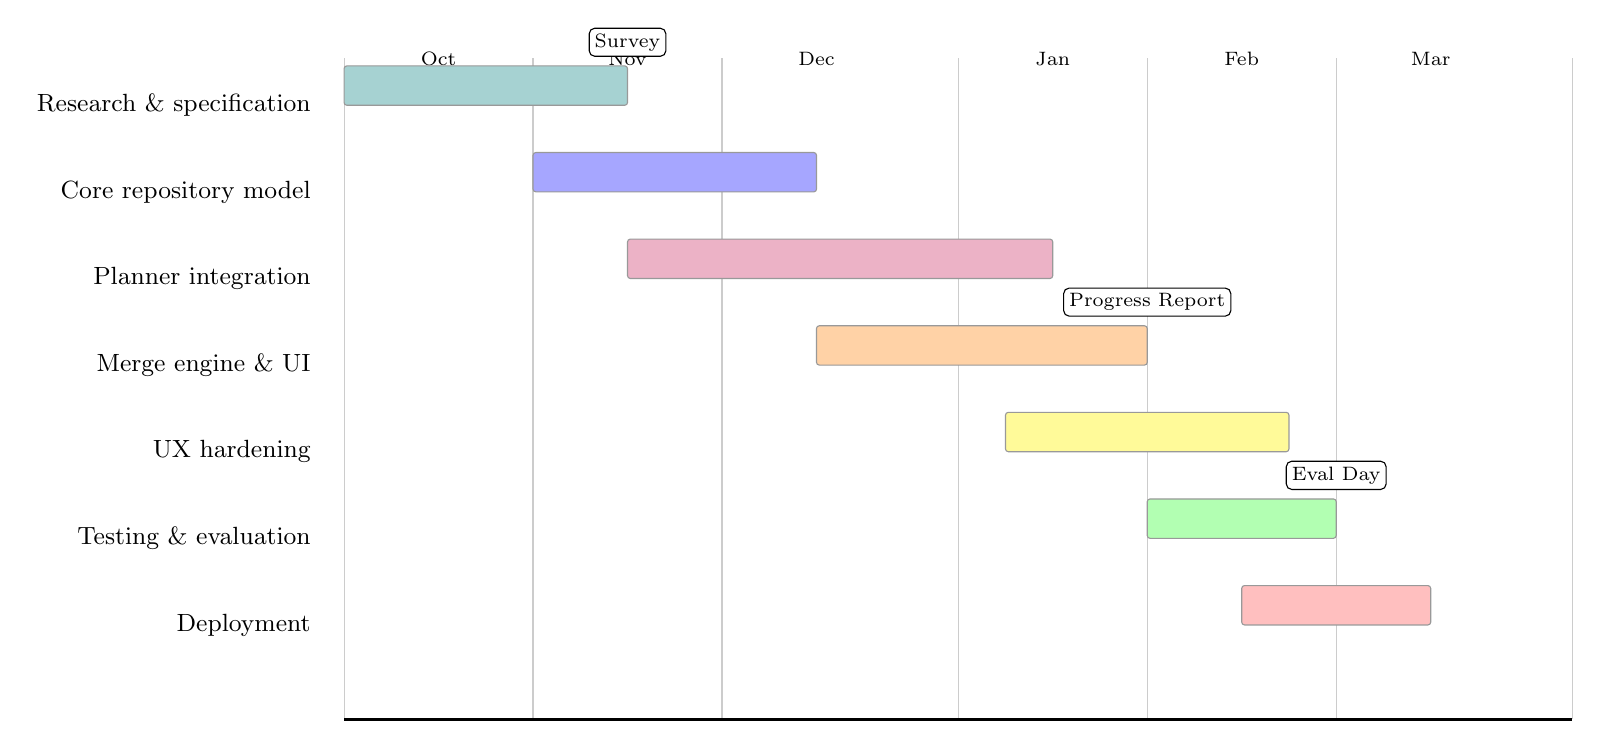
\begin{tikzpicture}[
    every node/.style={font=\small},
    bar/.style={fill=#1, draw=black!40, rounded corners=1pt, minimum height=0.5cm},
    bar/.default={blue!30},
    phaselabel/.style={font=\small, anchor=east},
    monthlabel/.style={font=\scriptsize, anchor=north},
  ]
    % Time axis: Oct 2025 to Mar 2026 = 6 months, 1cm per week (26 weeks)
    % Oct=4w, Nov=4w, Dec=4w, Jan=5w, Feb=4w, Mar=5w (approx)
    \def\wk{0.6}  % cm per week

    % Month boundaries (cumulative weeks)
    \def\octStart{0}
    \def\novStart{4}
    \def\decStart{8}
    \def\janStart{13}
    \def\febStart{17}
    \def\marStart{21}
    \def\totalWk{26}

    % Grid lines
    \foreach \m/\lbl in {\octStart/Oct,\novStart/Nov,\decStart/Dec,\janStart/Jan,\febStart/Feb,\marStart/Mar} {
      \draw[black!20] (\m*\wk, 0.6) -- (\m*\wk, -7.8);
      \node[monthlabel] at (\m*\wk + 2*\wk, 0.8) {\lbl};
    }
    \draw[black!20] (\totalWk*\wk, 0.6) -- (\totalWk*\wk, -7.8);

    % Phase bars (y positions)
    \def\yA{0}
    \def\yB{-1.1}
    \def\yC{-2.2}
    \def\yD{-3.3}
    \def\yE{-4.4}
    \def\yF{-5.5}
    \def\yG{-6.6}

    % Labels
    \node[phaselabel] at (-0.3, \yA) {Research \& specification};
    \node[phaselabel] at (-0.3, \yB) {Core repository model};
    \node[phaselabel] at (-0.3, \yC) {Planner integration};
    \node[phaselabel] at (-0.3, \yD) {Merge engine \& UI};
    \node[phaselabel] at (-0.3, \yE) {UX hardening};
    \node[phaselabel] at (-0.3, \yF) {Testing \& evaluation};
    \node[phaselabel] at (-0.3, \yG) {Deployment};

    % Bars: (start week * wk, y) rectangle (end week * wk, y + 0.5)
    % Research: Oct wk1 - Nov wk2 (weeks 0-6)
    \fill[bar=teal!35] (0*\wk, \yA) rectangle (6*\wk, \yA+0.5);
    % Core repo: Nov wk1 - Dec wk2 (weeks 4-10)
    \fill[bar=blue!35] (4*\wk, \yB) rectangle (10*\wk, \yB+0.5);
    % Planner: Nov wk3 - Jan wk2 (weeks 6-15)
    \fill[bar=purple!30] (6*\wk, \yC) rectangle (15*\wk, \yC+0.5);
    % Merge: Dec wk2 - Jan wk4 (weeks 10-17)
    \fill[bar=orange!35] (10*\wk, \yD) rectangle (17*\wk, \yD+0.5);
    % UX: Jan wk2 - Feb wk3 (weeks 14-20)
    \fill[bar=yellow!40] (14*\wk, \yE) rectangle (20*\wk, \yE+0.5);
    % Testing: Jan wk4 - Feb wk4 (weeks 17-21)
    \fill[bar=green!30] (17*\wk, \yF) rectangle (21*\wk, \yF+0.5);
    % Deployment: Feb wk2 - Mar wk2 (weeks 19-23)
    \fill[bar=red!25] (19*\wk, \yG) rectangle (23*\wk, \yG+0.5);

    % Milestone markers
    \node[font=\scriptsize, fill=white, draw=black, rounded corners=2pt,
          inner sep=2pt] at (6*\wk, \yA+0.5+0.3) {Survey};
    \node[font=\scriptsize, fill=white, draw=black, rounded corners=2pt,
          inner sep=2pt] at (17*\wk, \yD+0.5+0.3) {Progress Report};
    \node[font=\scriptsize, fill=white, draw=black, rounded corners=2pt,
          inner sep=2pt] at (21*\wk, \yF+0.5+0.3) {Eval Day};

    % Bottom axis
    \draw[thick] (0, -7.8) -- (\totalWk*\wk, -7.8);

  \end{tikzpicture}%
  }%
  \caption{Project Gantt chart showing the timeline for each development phase.
           Phases overlap where integration dependencies allowed parallel work.
           Key milestones are marked above the relevant bars.}
  \label{fig:gantt}
\end{figure}

\begin{table}[H]
\centering
\caption{Schedule detail: deliverables and status per phase.}
\label{tab:schedule_detail}
\begin{tabular}{@{}p{0.22\linewidth}p{0.55\linewidth}p{0.18\linewidth}@{}}
\toprule
\textbf{Phase} & \textbf{Deliverables} & \textbf{Status} \\
\midrule
Research \& specification & Competitor analysis; MoSCoW objectives; survey
  & Complete \\
Core repository model & Repos/branches/commits; snapshot storage
  & Complete \\
Planner integration & Routing matrix; ordering; constraints; spillover
  & Complete \\
Merge engine \& UI & Three-way merge; conflicts; resolver UI
  & Complete \\
UX hardening & Easy mode; discoverability; visual polish
  & Complete \\
Testing \& evaluation & Unit tests; UAT; survey analysis
  & Complete \\
Deployment & Containerisation; hosted instance; security checks
  & Complete \\
\bottomrule
\end{tabular}
\end{table}


\end{document}
